
% Document class and packages
\documentclass[12pt,a4paper,openany]{report}
\raggedbottom
\usepackage[utf8]{inputenc}
\usepackage[T1]{fontenc}
\usepackage[english]{babel}
\usepackage{amsmath,amsfonts,amssymb}
\usepackage{graphicx}
\usepackage{hyperref}
\usepackage{float}
\usepackage{longtable}
\usepackage[round]{natbib}
\usepackage{listings}
\usepackage[table]{xcolor}

\lstdefinestyle{pythonstyle}{
    language=Python,
    basicstyle=\ttfamily\small,
    keywordstyle=\color{blue},
    commentstyle=\color{gray},
    stringstyle=\color{teal},
    showstringspaces=false,
    breaklines=true,
    frame=single,
    numbers=left,
    numberstyle=\tiny\color{gray},
    captionpos=b
}
\let\parencite\citep
\let\textcite\citet

\newcommand{\ket}[1]{\lvert #1 \rangle}
\newcommand{\bra}[1]{\langle #1 \rvert}
\newcommand{\braket}[2]{\langle #1 \mid #2 \rangle}



% Remove blank pages between chapters
\let\cleardoublepage\clearpage

% Title and author information
\title{Quantifying quantumness: Determining the effect of quantum operations in machine learning models by comparison to classically simulatable variants}
\author{Víctor Mauricio Gutiérrez Luque\thanks{Computations were performed with computing resources granted by RWTH Aachen University under project \texttt{thes2204}.}}
\date{12.05.2026}
\begin{document}

% Title page
\begingroup
\renewcommand{\thefootnote}{}
\maketitle
\endgroup
\setcounter{footnote}{0}

% Abstract
\chapter*{Abstract}
\addcontentsline{toc}{chapter}{Abstract}
Quantum machine learning (QML) investigates whether quantum-mechanical representations and computations can improve machine-learning tasks. However, it is often unclear which observed performance differences are genuinely attributable to specifically quantum features rather than to architectural differences that can be implemented clasically or benchmarking effects. This thesis studies the role of entanglement in variational QML models through a controlled ablation or removal framework. The work introduces partially and fully separable variants of the Circuit-Centric Classifier (CCC) and IQP-Kernel Classifier, constructed by systematically reducing entangling interactions while keeping the remaining training and evaluation pipeline fixed. The models are evaluated on multiple synthetic and structured benchmark families, including but not limited to linearly separable, hidden-manifold, and hyperplane-based datasets. The results show that partially entangling variants often remain competitive with the original models, whereas fully separable variants typically exhibit larger performance degradation. The experiments are consistent with entanglement contributing meaningfully to performance in the studied models, while also suggesting that sparse entangling connectivity may already retain much of the observed benefit of the original architectures in this benchmark setting. The IQP-kernel experiments scaled prohibitively in higher-dimensional settings, exceeding the available computational budget.
\tableofcontents

% Chapters
\chapter{Introduction}

\section{Introduction and Related Literature}

Quantum machine learning sits at the intersection of quantum computing and statistical learning, and much of the literature has been motivated by the possibility that quantum models may represent or process patterns in ways that are classically difficult to reproduce. Foundational work on quantum feature maps, variational quantum circuits, and quantum kernels established the main model classes now used in the field \parencite{mitarai2018quantum,schuld2019evaluating,havlicek2019supervised,benedetti2019parameterized}. At the same time, more recent critical work has emphasized that the central scientific question is not simply whether a quantum model can outperform a classical baseline on a particular benchmark, but whether the observed behavior can actually be attributed to specifically quantum ingredients rather than to tuning choices, data selection, or architectural details that could also be reproduced classically \parencite{bowles2024better}.

This thesis is positioned within that second line of work. Rather than treating the presence of a quantum circuit as sufficient evidence of quantum advantage, it adopts an ablation-based view in which quantum models are compared to dequantized or classically simulable variants that differ in one controlled architectural feature. The focus here is entanglement. Entanglement is often regarded as one of the defining nonclassical resources of quantum computation, but in practical QML models it is not always clear whether it is genuinely responsible for predictive performance, or whether similar results can already be obtained with sparse or even fully local structures. The methodology of this thesis is therefore to reduce entanglement systematically while keeping the rest of the pipeline fixed.

The remainder of the document is structured as follows. Chapter~2 develops the background needed for the later analysis, including the basic quantum-computing formalism, core classical machine-learning concepts, the main QML model classes, and the benchmarking problem that motivates the study. Chapter~3 presents the experimental methodology, describes the benchmark families, defines the original and dequantized CCC variants, and outlines the corresponding IQP-kernel ablations together with the shared training and evaluation pipeline. Chapter~4 reports the empirical results, first quantitatively through ranking, forest, and accuracy plots, and then qualitatively through benchmark-family-level interpretation. Chapter~5 concludes by summarizing what the experiments show about entanglement in the studied models and by discussing possible directions for further work.


\chapter{Background}

\section{Quantum Computing Preliminaries}

\subsection{Behind Quantum Computing}
In the last century, there were measured results in classical physics giving absurdities. Initially, when people studied how hot objects glowed, the old theory predicted they should emit infinite amounts of UV light. Planck resolved this problem by proposing that energy is not exchanged continuously, but in discrete packets called quanta \parencite{planck_1900_blackbody}. Subsequently, the photoelectric effect showed that light can knock electrons out of metal only if its frequency is high enough; brightness or intensity of light alone did not help. Einstein explained this phenomenon by saying light behaves like particles (photons), each carrying one energy packet \parencite{einstein_1905_photoelectric}. A further development was Bohr's contribution. Atoms when heated were seen to emit only specific wavelengths or colors (spectral lines) and not a smooth rainbow. This made sense if electrons inside atoms can only have certain allowed energies. Bohr applied the quantum idea to atoms, proposing quantized energy levels for electrons in 1913, but without explaining why \parencite{bohr_1913_atom}. Consequently, De Broglie suggested that not only light, but also matter like electrons can act like waves; electron-diffraction experiments confirmed this \parencite{debroglie_1924_thesis}.

Heisenberg and Schr{\"o}dinger completed it by independently constructing new, self-consistent replacements for classical mechanics. Heisenberg started from the experimental fact that atomic spectra reveal only transitions between discrete energy levels. This led naturally to a matrix-based algebra in which the order of operations matters, capturing quantum behavior without relying on classical orbits. Schr{\"o}dinger, in contrast, searched for a wave equation governing microscopic systems of matter. This yielded correct bound-state energies and spectral predictions. They were soon shown to be mathematically equivalent descriptions of the same theory, and Born provided the probabilistic interpretation of the wavefunction \parencite{heisenberg_1925_matrix_mechanics,schrodinger_1926_wave_mechanics,born_1926_born_rule}. In short: classical physics failed for small-scale phenomena, and quantum mechanics was the new rulebook that fit the experiments.

In the classical computation model, information is encoded in bits and processed by deterministic or randomized operations, and the time and memory required by these operations determine what is computationally feasible. Quantum computing extends this model by introducing a new unit of information, the qubit, whose behavior follows the rules of quantum mechanics. Unlike a classical bit, which is always either 0 or 1, a qubit can occupy infinitely many states on a continuous state space; before measurement it can exist in a superposition of basis states; measurement irreversibly changes the qubit's state; and the outcome depends on the measurement basis, meaning the same qubit can be probed along many different axes \parencite{nielsen_chuang_qcqi}.

These features are valuable not because they allow unlimited extraction of information, but because they allow information to be encoded in complex amplitudes and phases, manipulated through continuous unitary transformations, and combined across qubits to produce interference and entanglement. 

Well-designed quantum algorithms exploit these effects so that, after a sequence of gates, the probability of measuring a desired result is amplified while unwanted outcomes are suppressed. These capabilities have no direct classical analogue. This mechanism is behind landmark quantum speedups such as Shor's algorithm for integer factoring and discrete logarithms, which runs in polynomial time on a quantum computer compared to the best known sub-exponential classical methods \parencite{shor_1994_focs,shor_1997_siam}, and Grover's algorithm for unstructured search, which reduces $O(N)$ classical query complexity to $O(\sqrt{N})$ using amplitude amplification \parencite{grover_1996_search}.

We will now first introduce the minimal linear-algebra language needed to describe quantum states and operations; then define qubits and single-qubit gates; extend to multi-qubit systems via tensor products and entanglement; and finally present the circuit model as the formal framework for quantum computation.

\subsection{Some Linear Algebra}

We briefly review the basic linear algebra concepts used throughout this thesis.\footnote{This overview is based on the exposition in \textcite[Chapter~2]{nielsen_chuang_qcqi}.}


A vector is a geometric object that as a magnitude and a direction and can live in a certain vector space, represented as columns whose values are in the domain. The basic operations are vector addition and scalar multiplication, and any expression of the form $\sum_i \alpha_i v_i$ is a linear combination of vectors $v_i$ with coefficients $\alpha_i$.

A map between vector spaces is linear if it respects these operations, $L(\alpha v + \beta w) = \alpha L(v) + \beta L(w)$. The standard Hermitian inner product is $\langle v,w\rangle = \sum_i \overline{v_i} w_i$, which induces the norm $\|v\| = \sqrt{\langle v,v\rangle}$. Two vectors are orthogonal if $\langle v,w\rangle = 0$, and a vector is normalized if $\|v\| = 1$. We often write vectors and inner products in bra--ket notation, where a column vector is denoted $\lvert v\rangle$, its conjugate transpose is $\langle v\rvert$, and the inner product is $\langle v \vert w\rangle$.

A basis $\{e_1,\dots,e_n\}$ of $\mathbb{C}^n$ is a set of vectors such that every vector has a unique coordinate representation $v = \sum_i \alpha_i e_i$; if, in addition, $\langle e_i,e_j\rangle = \delta_{ij}$, the basis is orthonormal. The standard (computational) basis of $\mathbb{C}^n$ consists of the unit vectors with a single $1$ in one position and $0$ elsewhere, and any vector can be written as a linear combination of these basis vectors.

Linear maps on the vector space are represented by matrices, and their action on a vector is given by matrix-vector multiplication; special directions that are only rescaled by a matrix are captured by eigenvectors $v$ with eigenvalues $\lambda$, satisfying $Av = \lambda v$. Of particular importance are unitary matrices $U$, defined by the condition $U^\dagger U = I$, where $U^\dagger$ is the conjugate transpose and $I$ is the identity. Unitary operators preserve inner products, and hence norms and angles, and are always reversible with inverse $U^{-1} = U^\dagger$.


\subsection{Postulates of Quantum Mechanics}


In this subsection we summarize the standard postulates of finite-dimensional quantum mechanics in the language of complex vector spaces introduced above. According more detailed discussion can be found in \textcite[Chapter~2]{nielsen_chuang_qcqi}.

\paragraph{Postulate 1 (State space).}
To every isolated physical system there corresponds a complex Hilbert space $\mathcal{H}$, called the state space of the system. The (pure) states of the system are represented by unit vectors $\lvert \psi \rangle \in \mathcal{H}$ with $\langle \psi \vert \psi \rangle = 1$. Two vectors that differ only by a nonzero complex scalar multiple represent the same physical state. In particular, $\lvert \psi \rangle$ and $e^{i\theta} \lvert \psi \rangle$ are physically indistinguishable for any real $\theta$.

\paragraph{Postulate 2 (Time evolution of closed systems).}
The time evolution of a closed system is described by a unitary operator on its state space. If the state at time $t_1$ is $\lvert \psi(t_1) \rangle$ and the state at time $t_2$ is $\lvert \psi(t_2) \rangle$, then there exists a unitary operator $U$ on $\mathcal{H}$ such that
\begin{equation}
  \lvert \psi(t_2) \rangle = U \lvert \psi(t_1) \rangle,
\end{equation}
where $U^\dagger U = I$. Unitary evolution preserves inner products and, in particular, the normalization of state vectors.

\paragraph{Postulate 3 (Measurement).}
Let $\{\lvert i \rangle\}$ be an orthonormal basis of the state space $\mathcal{H}$, and consider a measurement in this basis. Any state can be written as
\begin{equation}
  \lvert \psi \rangle = \sum_i \alpha_i \lvert i \rangle, \qquad \sum_i \lvert \alpha_i \rvert^2 = 1.
\end{equation}
The measurement has discrete outcomes labeled by $i$, and quantum mechanics assigns:
\begin{itemize}
  \item probability
  \begin{equation}
    p(i) = \lvert \alpha_i \rvert^2 = \lvert \langle i \vert \psi \rangle \rvert^2
  \end{equation}
  to obtaining outcome $i$;
  \item post-measurement state
  \begin{equation}
    \lvert \psi_i \rangle = \lvert i \rangle
  \end{equation}
  conditioned on observing outcome $i$.
\end{itemize}
Equivalently, this measurement can be described by the family of orthogonal projectors $P_i = \lvert i \rangle \langle i \rvert$, with $p(i) = \langle \psi \vert P_i \vert \psi \rangle$ and normalized post-measurement states $\lvert \psi_i \rangle = P_i \lvert \psi \rangle / \sqrt{p(i)}$. More general measurements can be modeled by a collection of measurement operators $\{M_m\}$ satisfying $\sum_m M_m^\dagger M_m = I$, but in this thesis we will primarily use projective measurements in the computational basis.

\paragraph{Postulate 4 (Composite systems).}
For a composite system consisting of subsystems $A$ and $B$ with state spaces $\mathcal{H}_A$ and $\mathcal{H}_B$, the state space of the combined system is the tensor product
\begin{equation}
  \mathcal{H}_{AB} = \mathcal{H}_A \otimes \mathcal{H}_B.
\end{equation}
If $\lvert \psi \rangle_A \in \mathcal{H}_A$ and $\lvert \phi \rangle_B \in \mathcal{H}_B$ are states of the individual subsystems, then the product state of the composite system is $\lvert \psi \rangle_A \otimes \lvert \phi \rangle_B$. More generally, a pure state of the composite system is any unit vector $\lvert \Psi \rangle_{AB} \in \mathcal{H}_A \otimes \mathcal{H}_B$, which can be expressed as
\begin{equation}
  \lvert \Psi \rangle_{AB} = \sum_{ij} \alpha_{ij} \lvert i \rangle_A \otimes \lvert j \rangle_B
\end{equation}
with respect to chosen orthonormal bases $\{\lvert i \rangle_A\}$ and $\{\lvert j \rangle_B\}$.
A pure state is called \emph{separable} if it can be written as $\lvert \Psi \rangle_{AB} = \lvert \psi \rangle_A \otimes \lvert \phi \rangle_B$ for some $\lvert \psi \rangle_A$ and $\lvert \phi \rangle_B$, otherwise \emph{entangled}.
Even when entangled qubits are spatially separated, a measurement on one qubit instantaneously fixes the conditional state of the others: once an outcome is obtained on one side, the outcome probabilities on the other side are updated accordingly.
For example, if
\[
|\psi\rangle = \begin{pmatrix} a \\ b \end{pmatrix}, \quad |\phi\rangle = \begin{pmatrix} c \\ d \end{pmatrix},
\]
then their tensor product is:
\[
|\psi\rangle \otimes |\phi\rangle = \begin{pmatrix} a c \\ a d \\ b c \\ b d \end{pmatrix}.
\]

\subsection{Quantum Computing}

Classical computers represent information using \textit{bits}, which can take values of either 0 or 1. Quantum computing generalizes this idea using \textit{quantum bits}, or \textit{qubits}.

A single qubit is a two-dimensional quantum system with state space $\mathcal{H} \cong \mathbb{C}^2$. Fixing the computational basis $\{\ket{0},\ket{1}\}$, any pure state of a qubit can be written as
\begin{equation}
  \ket{\psi} = \alpha \ket{0} + \beta \ket{1}, \qquad \alpha,\beta \in \mathbb{C}, \quad \lvert \alpha \rvert^2 + \lvert \beta \rvert^2 = 1.
\end{equation}
As global phases are irrelevant, because $\ket{\psi}$ and $e^{i\theta}\ket{\psi}$ describe the same physical state, we can use this to parametrize any qubit state by two real angles $\theta \in [0,\pi]$ and $\varphi \in [0,2\pi)$ as
\begin{equation}
  \ket{\psi(\theta,\varphi)} = \cos\!\left(\frac{\theta}{2}\right)\ket{0}
  + e^{i\varphi} \sin\!\left(\frac{\theta}{2}\right)\ket{1}.
\end{equation}
The pair $(\theta,\varphi)$ can be interpreted as spherical coordinates of a point on the unit sphere in $\mathbb{R}^3$. This represents the \emph{Bloch sphere}: every qubit state corresponds to a point on the surface of the sphere, with $\ket{0}$ and $\ket{1}$ at the north and south poles, respectively.


Unitary operators preserve inner products and norms, so they map pure states to pure states, corresponding to rotations. 

A \emph{single-qubit gate} is such a unitary operation applied to an individual qubit. Important examples include the Pauli operators
\begin{equation}
  X = \begin{pmatrix} 0 & 1 \\ 1 & 0 \end{pmatrix}, \quad
  Y = \begin{pmatrix} 0 & -i \\ i & 0 \end{pmatrix}, \quad
  Z = \begin{pmatrix} 1 & 0 \\ 0 & -1 \end{pmatrix},
\end{equation}
which generate $\pi$-rotations about the $x$-, $y$-, and $z$-axes of the Bloch sphere. The Pauli-$X$ gate exchanges $\ket{0}$ and $\ket{1}$ and is the quantum analogue of a classical NOT gate. The Pauli-$Z$ gate leaves $\ket{0}$ invariant and multiplies $\ket{1}$ by a phase $-1$, thereby changing relative phase without altering the measurement probabilities in the computational basis.

Another fundamental gate is the Hadamard operator
\begin{equation}
  H = \frac{1}{\sqrt{2}}\begin{pmatrix} 1 & 1 \\ 1 & -1 \end{pmatrix},
\end{equation}
which maps basis states to equal superpositions,
\begin{equation}
  H\ket{0} = \frac{\ket{0} + \ket{1}}{\sqrt{2}}, \qquad
  H\ket{1} = \frac{\ket{0} - \ket{1}}{\sqrt{2}}.
\end{equation}
The Hadamard gate is routinely used to create superposition states from computational basis states. More generally, one often considers continuous families of \emph{rotation gates}
\begin{equation}
  R_X(\theta) = e^{-i\theta X/2}, \quad
  R_Y(\theta) = e^{-i\theta Y/2}, \quad
  R_Z(\theta) = e^{-i\theta Z/2},
\end{equation}
which implement rotations of the Bloch vector by an angle $\theta$ around the corresponding axis, as well as phase gates such as
\begin{equation}
  S = \begin{pmatrix} 1 & 0 \\ 0 & i \end{pmatrix}, \qquad
  T = \begin{pmatrix} 1 & 0 \\ 0 & e^{i\pi/4} \end{pmatrix},
\end{equation}
which modify the relative phase between $\ket{0}$ and $\ket{1}$.

To describe multiple qubits within the formalism of Postulate~4, we use the tensor product to build composite systems. If each single qubit lives in a two-dimensional Hilbert space $\mathcal{H} \cong \mathbb{C}^2$ with basis $\{\ket{0},\ket{1}\}$, then the state space of an $n$-qubit register is the tensor product
\begin{equation}
  \mathcal{H}^{\otimes n} = \underbrace{\mathcal{H} \otimes \cdots \otimes \mathcal{H}}_{n \text{ times}} \cong \mathbb{C}^{2^n}.
\end{equation}
The computational basis of $\mathcal{H}^{\otimes n}$ consists of all $2^n$ tensor products of single-qubit basis states,
\begin{equation}
  \{\ket{x_1}\otimes \cdots \otimes \ket{x_n} : x_k \in \{0,1\}\},
\end{equation}
which are usually written more compactly as $\ket{x_1\cdots x_n}$ for $x_1\cdots x_n \in \{0,1\}^n$. Any pure $n$-qubit state can be expressed as a linear combination
\begin{equation}
  \ket{\Psi} = \sum_{x \in \{0,1\}^n} \alpha_x \ket{x}, \qquad \sum_{x} \lvert \alpha_x \rvert^2 = 1.
\end{equation}

A particularly simple class of multi-qubit states are \emph{product states}, which factorize as a tensor product of single-qubit states, for example
\begin{equation}
  \ket{\Psi} = \ket{\psi_1} \otimes \cdots \otimes \ket{\psi_n},
\end{equation}
with each $\ket{\psi_k} = \alpha_k \ket{0} + \beta_k \ket{1}$. However, Postulate~4 allows more general states that cannot be written in this factorized form, entangled states. Popular examples are the Bell states, such as
\begin{equation}
  \ket{\Phi^+} = \frac{1}{\sqrt{2}}\big(\ket{00} + \ket{11}\big).
\end{equation}

Measuring the first qubit of $\ket{\Phi^+}$ in the computational basis yields outcome $0$ or $1$ with equal probability, but conditioned on the outcome, the state of the second qubit is perfectly correlated: if the first outcome is $0$ the joint state collapses to $\ket{00}$, whereas if the first outcome is $1$ it collapses to $\ket{11}$. These correlations cannot be explained by any classical product state and are stronger than those obtainable from independent systems with shared classical randomness.

Entanglement plays a central role in quantum computation because it allows a quantum computer to represent and manipulate correlations across many subsystems in a way that has no direct classical analogue. In an $n$-qubit register, generic pure states live in a space of dimension $2^n$, and entangled states can encode joint amplitude patterns over all $2^n$ basis strings. 

It is important to distinguish entanglement from superposition. Superposition already appears at the single-qubit level: a state of the form $\ket{\psi} = \alpha\ket{0} + \beta\ket{1}$ is a superposition of basis states, but not entangled, because it concerns only one system. Every entangled state is also a superposition, but not every superposition is entangled. 

A quantum circuit consists of a sequence of quantum gates acting on a register of qubits. The structure of a quantum circuit reflects the algorithmic logic of the computation, with qubits initialized in known basis states, processed through a network of gates, and finally measured to extract classical information. Quantum algorithms exploit this structure by applying multi-qubit gates that create and transform entanglement, so that interference between many computational paths can be steered towards desired outcomes.

\subsubsection{Grover's Algorithm}

To illustrate the operation of a quantum circuit, consider Grover’s algorithm \parencite{grover_1996_search}, which provides a quadratic speedup for the problem of searching an unstructured database. 
Grover's algorithm works as followed: given a function \( f: \{0,1\}^n \rightarrow \{0,1\} \) that evaluates to \( f(x) = 1 \) for a unique input \( x = x_0 \), and \( f(x) = 0 \) otherwise, the goal is to find \( x_0 \). Classically, this requires \( \mathcal{O}(2^n) \) evaluations in the worst case, whereas Grover's algorithm achieves this in \( \mathcal{O}(\sqrt{2^n}) \) steps.

\begin{figure}[htbp]
    \centering
    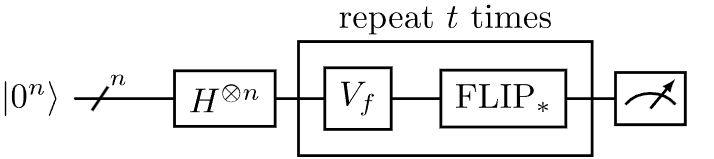
\includegraphics[width=0.75\linewidth]{figures/grover_circuit.png}
    \caption{The quantum circuit for Grover’s algorithm}
    \label{fig:grover-circuit}
\end{figure}

\begin{enumerate}
    \item \textbf{Initialization}

    We begin with an \( n \)-qubit register initialized to the state \( \ket{0}^{\otimes n} \). Applying the Hadamard transform \( H^{\otimes n} \) yields the uniform superposition:

    \[
    \ket{\psi} = \frac{1}{\sqrt{N}} \sum_{x \in \{0,1\}^n} \ket{x}, \quad \text{where } N = 2^n.
    \]

    This state assigns equal probability amplitude to every possible input \( x \in \{0,1\}^n \).

    \item \textbf{Oracle Operator}

    The oracle \( V_f \) is a unitary operator that flips the sign of the amplitude of the solution \( x_0 \). Formally:

    \[
    V_f \ket{x} = 
    \begin{cases}
    - \ket{x} & \text{if } x = x_0, \\
    \phantom{-} \ket{x} & \text{otherwise}.
    \end{cases}
    \]

    This phase inversion does not reveal \( x_0 \), but encodes its identity into the quantum state.

   \item \textbf{Diffusion Operator or $\text{FLIP}_{*}$}

    The diffusion operator, often referred to as the inversion about the average, amplifies the probability amplitude of the solution. It is defined as:

    \[
    D = 2 \ket{\psi}\bra{\psi} - I,
    \]

    where \( \ket{\psi} \) is the initial uniform superposition and \( I \) is the identity matrix. When applied to a state \( \ket{\phi} \), the operator reflects \( \ket{\phi} \) about \( \ket{\psi} \).

    \item \textbf{Grover Iteration}

    One Grover iteration consists of applying the oracle followed by the diffusion operator:

    \[
    G = D \cdot V_f.
    \]

    The state after \( t \) iterations is:

    \[
    \ket{\psi^{(t)}} = G^t \ket{\psi}.
    \]

    It can be shown that each application of \( G \) rotates the state vector closer toward the solution state \( \ket{x_0} \) in a two-dimensional subspace spanned by \( \ket{x_0} \) and its orthogonal complement. The rotation angle \( \theta \) satisfies:

    \[
    \cos(\theta) = \sqrt{\frac{N - 1}{N}}, \quad \text{so } \theta \approx \frac{1}{\sqrt{N}} \text{ for large } N.
    \]

    To maximize the probability of measuring \( x_0 \), the number of iterations should be approximately:

    \[
    t = \left\lfloor \frac{\pi}{4} \sqrt{N} \right\rfloor.
    \]

    \item \textbf{Measurement and Success Probability}

    After applying \( t \) iterations, we measure the quantum state in the computational basis. With high probability (approaching 1 as \( N \to \infty \)), the outcome will be the desired value \( x_0 \). The overall complexity of the algorithm is therefore \( \mathcal{O}(\sqrt{N}) \), providing a quadratic speedup over classical brute-force search.
\end{enumerate}

\section{Classical Machine Learning}
Supervised learning is a core approach in machine learning in which the goal is to infer a mapping from inputs to outputs using a dataset of labeled examples. Each example is represented as a pair $(\mathbf{x}, y)$, where $\mathbf{x} \in \mathbb{R}^n$ is an input vector composed of $n$ features, and $y$ is the corresponding target value. The learning algorithm or mathematical function, the model, attempts to approximate a function $f: \mathbb{R}^n \rightarrow \mathcal{Y}$ that best predicts $y$ given $\mathbf{x}$, where \(\mathcal{Y}\) denotes the set of all possible target values, also called the output or label space \parencite{murphy2012}.


Some models in supervised learning are called \textit{parametric}, meaning they assume a fixed form for the function $f$ and learn a set of parameters, typically denoted by a weight vector \(\mathbf{w} \in \mathbb{R}^n\)  and a bias term \(b \in \mathbb{R}\) during training. Others are \textit{non-parametric}, which means their structure or complexity grows with the amount of data, without assuming a fixed number of parameters \parencite{murphy2012}.


In classification tasks, models often produce an intermediate output $z = \mathbf{w}^\top \mathbf{x} + b$, called the score. This  is a real-valued scalar that serves as a bridge between raw input features through a decision or \textit{activation function} to final output labels \( \hat{y} \in \mathcal{Y} \). For example, a \textit{sign function} \( \hat{y} = \text{sign}(z)\) returns $+1$ or $-1$ based on the sign of $z$, while probabilistic models may use sigmoid or softmax functions to produce class probabilities. The geometry and dimensionality of the feature space (i.e., how many and which features are used to describe each $\mathbf{x}$) deeply influence how models learn and generalize.

\subsection{Linear Classifiers}
Linear classifiers are a class of models that separate data points in a feature space using a hyperplane defined by a weight vector $\mathbf{w} \in \mathbb{R}^n$ and a scalar bias term $b \in \mathbb{R}$. The model computes a linear combination $z = \mathbf{w}^\top \mathbf{x} + b$, and the sign of $z$ determines the predicted class. This leads to a decision function of the form $f(\mathbf{x}) = \text{sign}(\mathbf{w}^\top \mathbf{x} + b)$, where $\text{sign}(\cdot)$ returns $+1$ for positive inputs and $-1$ for negative ones \parencite{rosenblatt1958}.

The vector $\mathbf{w}$ encodes the relative importance of each feature in the input $\mathbf{x}$, while the bias $b$ shifts the decision boundary. The decision boundary itself is the set of points $\mathbf{x}$ for which $\mathbf{w}^\top \mathbf{x} + b = 0$. Linear classifiers rely on the assumption that classes can be separated by such a boundary in the input space \parencite{rosenblatt1958}. They form the basis of many more complex models and are computationally simple, making them a foundational concept in machine learning.

\subsection{Support Vector Machine (SVM)}
While linear classifiers separate the classes by finding any line, which makes them sensitive to outliers, support vector machines (SVMs) \parencite{cortes1995svm}, by construction, are margin-based classifiers that aim to find the hyperplane separating two classes, and not focus on outlier points. This makes them more outlier-robust. Given training examples labeled $y_i \in \{-1, +1\}$, the SVM solves an optimization problem that finds the hyperplane $\mathbf{w}^\top \mathbf{x} + b = 0$ such that the distance between this hyperplane and the closest data points (called \textit{support vectors}) is maximized.

Maximizing the margin improves the model’s robustness to variations in the data. The supporting hyperplanes, those defining the margin boundaries, are given by \( w^T x + b = \pm 1 \). The distance from the decision boundary to each of these hyperplanes is \( \frac{1}{\|w\|} \). Therefore, the total margin width, which is the distance between the two margin hyperplanes, is \( \frac{2}{\|w\|} \). Maximizing it is equivalent to minimizing $\|\mathbf{w}\|^2$, which leads to the primal optimization formulation. This choice regularizes the model by penalizing large weights, which in turn reduces sensitivity to small fluctuations in input values.

The model predicts labels using the \textit{sign function}: $f(\mathbf{x}) = \text{sign}(\mathbf{w}^\top \mathbf{x} + b)$. In this setting, the sign of the inner product determines on which side of the hyperplane the input lies. If the data are not linearly separable, SVMs can be extended using kernel functions, which allow the model to behave as if the data were mapped into a higher-dimensional space, where a linear separator may exist, without explicitly computing that mapping.


\subsection{Kernel Methods }
Kernel methods \parencite{scholkopf2002learning} are a set of techniques that allow linear models to learn non-linear patterns by computing similarities between data points using a \textit{kernel function}. A kernel is a function $K(\mathbf{x}, \mathbf{x}')$ that measures how similar two inputs are, without explicitly mapping them into a higher-dimensional space. Instead, it leverages the mathematical property that inner products in this high-dimensional space can be computed directly via the kernel, a concept known as the \textit{kernel trick}.

One widely used kernel is the Gaussian kernel or RBF(Radial Basis Function):
\[
K(\mathbf{x}, \mathbf{x}') = \exp\left(-\frac{\|\mathbf{x} - \mathbf{x}'\|^2}{2\sigma^2}\right)
\]
This function assigns high similarity to points that are close in Euclidean space and low similarity to distant points. This similarity measure enables the model to construct complex, non-linear decision boundaries in the input space, while still solving a linear problem in an implicit feature space.


\subsection{Neural Networks (MLPs)}
Multilayer Perceptrons (MLPs) \parencite{goodfellow2016deep} are a class of feedforward neural networks consisting of multiple layers of \textit{artificial neurons}. Each neuron computes a weighted sum of its inputs, applies a non-linear \textit{activation function} such as the rectified linear unit (ReLU), sigmoid, or hyperbolic tangent (tanh), and passes the result to the next layer. An MLP typically consists of an \textit{input layer}, one or more \textit{hidden layers}, and an \textit{output layer}.

Formally, each hidden layer performs a transformation of the form:
\[
\mathbf{h}^{(l)} = \sigma(\mathbf{W}^{(l)} \mathbf{h}^{(l-1)} + \mathbf{b}^{(l)})
\]
where $\mathbf{W}^{(l)}$ and $\mathbf{b}^{(l)}$ are the weights and biases of layer $l$, and $\sigma(\cdot)$ is the activation function. The model is trained using \textit{backpropagation}, which computes gradients of a loss function with respect to each parameter using the chain rule, followed by \textit{gradient descent} to update the weights.

Small MLPs, typically with one or two hidden layers and a moderate number of units, are capable of learning complex, non-linear relationships while maintaining tractability. Unlike kernel methods or instance-based models, MLPs \textit{learn internal representations} of the data during training, which makes them a flexible and general-purpose modeling approach.

\paragraph{Convolutional Neural Networks (CNNs).}
For image-like data, a common variant of neural networks is the convolutional neural network (CNN). 
Instead of fully connecting every input pixel to every neuron in the first layer, CNNs use \emph{convolutional layers}, which apply small learnable filters locally across the input. 
The same filter is reused at all spatial positions, so the network can detect the same pattern (edges, lines or corners) regardless of where it appears in the image. 
Convolutional layers are typically followed by non-linear activation functions and \emph{pooling} operations that downsample the feature maps, gradually reducing spatial resolution while increasing the level of abstraction. 
In the final stages, one or more fully connected layers map these extracted features to class scores, making CNNs particularly effective for image classification tasks.


\section{Quantum Machine Learning}

\subsection{How data is encoded?}

Classical data can be embedded into quantum states in several ways; here we briefly
summarise a few common schemes following \textcite{rath2023quantum}.

\paragraph{Basis (computational) encoding.}
The most direct method maps each classical bit to a qubit in the computational basis.
A classical bit string such as $101$ is represented as the basis state
\[
    |101\rangle = |1\rangle \otimes |0\rangle \otimes |1\rangle .
\]
If we measure in the computational basis, we always obtain the string $101$; the
information is stored in \emph{which} basis state the system occupies.

\paragraph{Superposition encoding.}
Instead of a single basis state, one can encode information in a superposition of
several classical strings. For example,
\[
    |\psi\rangle = \frac{1}{\sqrt{3}}\bigl(|100\rangle + |010\rangle + |001\rangle\bigr)
\]
encodes that the system is in one of the three strings $100$, $010$, or $001$
with equal probability. Measurement yields one of these outcomes with probability
$1/3$, so the information is contained in which basis states appear and with which
amplitudes.

\paragraph{Angle encoding.}
In angle (or rotation) encoding, real-valued features are used as rotation angles on
single qubits. For a two-dimensional data point $x = (x_1,x_2)$, one can prepare
\[
    |\psi(x)\rangle
    = R_y(x_1)\otimes R_y(x_2)\,|00\rangle
    = R_y(x_1)|0\rangle \otimes R_y(x_2)|0\rangle ,
\]
where $R_y(x)$ is a rotation about the $y$-axis by angle $x$. The measurement
probabilities then depend smoothly on the input values $x_1$ and $x_2$. Analogy: each qubit is an arrow on the Bloch sphere. Your data tells you how much to turn the arrow.

\paragraph{Amplitude encoding.}
Amplitude encoding uses the components of a (normalised) classical vector as the
amplitudes of a quantum state. For instance, for $x = (1,2,0,1)$ we first normalise
$\|x\| = \sqrt{1^2 + 2^2 + 0^2 + 1^2} = \sqrt{6}$ and prepare the two-qubit state
\[
    |\psi(x)\rangle
    = \frac{1}{\sqrt{6}}|00\rangle
      + \frac{2}{\sqrt{6}}|01\rangle
      + 0\cdot|10\rangle
      + \frac{1}{\sqrt{6}}|11\rangle .
\]
Here the classical information is encoded directly in the probability amplitudes of
each basis state. The classical numbers (1,2,0,1) decide how likely each basis state is, after the normalisation.

\subsection{Ansatz: How is the model learning?}

After encoding, the quantum state is processed by a variational ansatz, 
i.e.\ a quantum circuit \(U_{\mathrm{var}}(\theta)\) with a fixed gate
layout and fixed parameters or trainable angles \(\theta\). The ansatz specifies how many layers of
single-qubit rotations and entangling gates are used, on which qubits they act,
and how the qubits are connected. In this sense, it plays a role analogous to
the architecture of a classical neural network: choosing the number of layers,
the width of each layer, and the connectivity between neurons. While the feature
map determines how the classical input \(x\) is embedded into the Hilbert space,
the ansatz provides the trainable degrees of freedom that are optimized during
learning and thus defines the family of functions that the model
can represent \parencite{benedetti2019parameterized}.

\subsection{Models in Quantum Machine Learning}
Following the models introduced in \parencite{bowles2024better}, we now discuss the following:
\subsubsection{VQC's: Variational Quantum Circuits}

In the setting of quantum machine learning, variational quantum circuits or VQC's are often
described abstractly as functions of the form
\[
    f(\theta, x) = \operatorname{tr}\!\big[ O(x,\theta)\,\rho(x,\theta) \big],
\]
where \(\rho(x,\theta)\) is a density matrix and \(O(x,\theta)\) is an observable.
This expression can be understood operationally as a three–step procedure.
First, a feature map (encoding circuit) \(U_{\mathrm{enc}}(x)\) prepares a
data-dependent quantum state from a simple initial state \(\rho_0\), for example
\(|0\ldots 0\rangle\langle 0\ldots 0|\). This yields the encoded state
\(U_{\mathrm{enc}}(x)\,\rho_0\,U_{\mathrm{enc}}(x)^{\dagger}\).
Second, a variational ansatz \(U_{\mathrm{var}}(\theta)\), i.e.\ a parametrized
quantum circuit with fixed gate layout and trainable angles \(\theta\), is applied
to this encoded state. The result is the joint data- and parameter-dependent state, or the density matrix,
\[
    \rho(x,\theta)
    = U_{\mathrm{var}}(\theta)\,U_{\mathrm{enc}}(x)\,\rho_0\,
      U_{\mathrm{enc}}(x)^{\dagger}U_{\mathrm{var}}(\theta)^{\dagger}.
\]
Finally, one measures a suitable observable \(O(x,\theta)\) on this state.
The scalar output is given by the trace or  \(f(\theta,x)\)=\(\operatorname{tr}[O(x,\theta)\rho(x,\theta)]\),
which is the expectation value of the measurement and serves as the prediction of
the quantum model for input \(x\) and parameters \(\theta\).

\subsubsection{Quantum Neural Networks}

We view a quantum neural network as in \parencite{bowles2024better} as a model that uses one or more
variational quantum circuits \(f_1,\dots,f_L\) and combines their scalar outputs
through a classical prediction function \(f_{\mathrm{pred}}\) to produce a binary
label \(y \in \{\pm 1\}\):
\[
    y = f_{\mathrm{pred}}\bigl(f_1(\theta_1,x),\dots,f_L(\theta_L,x)\bigr).
\]

In the simplest case, we use only one quantum circuit (\(L = 1\)) and measure an
operator whose possible outcomes are \(-1\) or \(+1\). The circuit output is then
a number between \(-1\) and \(+1\) (its expectation value), and we choose the
predicted class just by its sign: a positive value means class \(+1\), while a
negative value means class \(-1\).

Training proceeds analogously to classical neural networks. Given a dataset
\(\{(x_i,y_i)\}_{i=1}^N\), we define an average loss as
\[
    \mathcal{L}(\theta; X, y)
    = \frac{1}{N}\sum_{i=1}^N \ell\bigl(\theta, x_i, y_i\bigr),
\]
where \(\ell(\theta,x_i,y_i)\) is a pointwise loss and \((X,y\))
collect all inputs and labels. The parameters
\(\theta = (\theta_1,\dots,\theta_L)\) are then optimised using stochastic
gradient descent or related methods. Gradients with respect to quantum circuit
parameters are obtained via the chain rule and parameter-shift rules \parencite{mitarai2018quantum,schuld2019evaluating}.


\subsubsection{Quantum Kernel Methods}

Quantum kernel methods adapt classical kernel-based learning (such as support
vector machines) to the quantum setting by using a quantum device to define and
evaluate the kernel function. The key idea is to embed each classical data point
\(x\) into a quantum state \(\rho(x)\) via a feature map (encoding circuit), and
to define the kernel as an inner product between such states, for example
\[
    k(x_i, x_j) = \operatorname{tr}\big[\rho(x_i)\,\rho(x_j)\big].
\]
This quantum kernel can then be plugged into a standard classical kernel
algorithm, which operates exactly as in the classical case but now uses
similarities computed by a quantum circuit. In this way, the “model” remains a
classical kernel method, while the quantum computer is used only to realise a
potentially rich feature space that may be hard to simulate classically.






\section{Motivation: The Benchmarking Problem in QML}

\subsection{The benchmarking problem in quantum machine learning}
\label{subsec:benchmarking-qml}

Before large, fault-tolerant quantum computers are available, almost all empirical evidence about quantum machine learning (QML) comes from classical simulations of small quantum models or from experiments on noisy, few-qubit devices. In this regime, \emph{benchmarking}, systematically comparing quantum models against each other and against classical baselines on common tasks, is one of the few tools available to assess whether current ideas in QML actually deliver on their promised advantages, as discussed in \textcite{bowles2024better}. 

However, as \textcite{bowles2024better} argue, drawing robust conclusions from such benchmarks is surprisingly difficult: small design choices in datasets, model architectures, metrics, and hyperparameter tuning can drastically change which model ``wins''. This makes it hard to answer even seemingly simple questions such as whether a given quantum model is ``better than'' a classical one.

\begin{itemize}
  \item \textbf{Dataset choice has a huge impact.}  
  Classical ``no free lunch'' results already tell us that average performance of any learning algorithm depends strongly on the distribution of tasks considered. In practice, this means that simply changing which datasets are included in a benchmark, or how they are preprocessed, can completely reorder the ranking of methods. Empirically, even for standard classical models, fixing label errors in a dataset, changing the train--test split, or switching to a different evaluation metric can significantly shift which model appears best. In the QML setting, where many studies rely on only one or two small datasets, this sensitivity is even more problematic. Papers that illustrate this effect include
\parencite{dehghani2021benchmarklottery,northcutt2021pervasive,recht2018cifar10,recht2019imagenet}.

  
  \item \textbf{Benchmark design embeds many hidden choices.}  
  Beyond the data itself, numerous ``small'' design decisions shape the outcome:
  \begin{itemize}
    \item Architectural tweaks (new ansätze, exotic layers, etc.) are often advertised as innovations, but large-scale benchmarks suggest that they frequently have little consistent effect on performance.
    \item Hyperparameter optimisation (learning rates, layer counts, regularisation, kernel parameters, etc.) typically dominates performance: with enough tuning, a simple baseline can match or surpass more elaborate proposals.
    \item Different evaluation metrics (accuracy, F1-score, AUC, calibration measures, or cost-sensitive scores) reward different behaviour and may correlate poorly, so ``best'' can mean different things depending on what is measured.
    \item When computational cost is taken into account (e.g., training time, circuit evaluations, required hardware or simulator resources), rankings can reverse: a slightly more accurate model may be clearly inferior when efficiency is factored in.
  \end{itemize}
  For QML, these issues are amplified because each circuit evaluation is expensive and gradients can require thousands of shots or full-state simulations, so hyperparameter searches are hardware- and time-intensive. Papers that illustrate this effect include
\parencite{narang2021transformer,smith2023convnets,lucic2018gans,henderson2018deeprlmatters,riquelme2018deepbayesianbandits,dodge2019showyourwork}.

  
  \item \textbf{Systematic positivity bias in the literature.}  
  A simple thought experiment illustrates how publication practices may create a risk of positivity bias: suppose many research groups each try a large number of quantum models and datasets, but only submit papers when they find a configuration where the quantum model outperforms a classical baseline. Even if, on average, classical models tend to do better, the literature will still be dominated by positive results that claim ``quantum beats classical''. This creates a misleading impression of steady progress, even if the underlying picture is much more mixed.
\end{itemize}

The conclusion is that broad questions of the form ``Are quantum models better than classical ones?'' cannot be answered by isolated experiments on a handful of small datasets. Instead, what can be meaningfully asked are \emph{narrow}, well-specified questions: for example, how the performance of a particular family of quantum models changes as a controlled difficulty parameter increases, or how sensitive a given ansatz is to noise, or how a quantum kernel compares to a specific classical kernel on a particular class of tasks. 

Carefully designed benchmarks must therefore emphasise controlled variation, reproducibility, and ablation-style comparisons over simple leaderboard rankings.

\paragraph{What matters in a comparison?}

Given these challenges, \textcite{bowles2024better} argue that benchmarking should move beyond simplistic leaderboard questions and instead ask \emph{structural} questions about model design. Rather than only asking whether a quantum model outperforms a classical baseline, we should try to understand \emph{which parts} of the model are crucial and which can be replaced by classically simulable components without loss of performance. In other words, benchmarking should be used as an \emph{ablation tool} to probe the role of quantum resources.

Concretely, they propose constructing ``dequantised'' variants of QML models by systematically removing or restricting those ingredients that are specifically quantum, for example by
\begin{itemize}
  \item removing entangling gates and using only local, single-qubit rotations (seen in the paper),
  \item restricting the gate set to Clifford transformations,
  \item replacing unitary evolutions by stochastic, or
  \item simulating circuits with tensor-network methods such as Matrix Product States (MPS) with low bond dimension.
\end{itemize}
By comparing the original model to these non-quantum or classically tractable variants on the \emph{same} benchmarks, one can probe to what extent genuine quantum effects are responsible for any observed performance differences. When a dequantised variant matches the original model, this suggests that ``quantumness'' was not the decisive ingredient, at least on the tasks and scales considered.


Motivated by this perspective, the present work adopts a similar philosophy. Rather than taking the presence of quantum circuits as evidence of a quantum advantage, we use benchmarking as a tool to dissect our models. After introducing baseline variational quantum classifiers, we will \emph{remove} its specifically quantum features and study how performance changes. In particular, we investigate variants following the dequantisation strategies suggested by \textcite{bowles2024better}. By comparing the original and dequantised models on controlled benchmarks, our goal is to understand not only \emph{how well} they perform, but also \emph{which aspects of their design appear most dependent on quantum resources}.



\chapter{Methodology}
\label{chap:methodology}

This chapter describes the experimental setup used to study the role of entanglement in two quantum model families: the Circuit-Centric Classifier (CCC) and the IQP kernel classifier. The main goal is not only to compare models by final accuracy, but to construct controlled ablations of each architecture and examine how performance changes as entanglement is reduced. To keep the comparison as fair as possible, all variants are evaluated within the same benchmarking framework, on the same datasets, and under the same training and hyperparameter-search procedure.

\section{Experimental Setup}

All experiments are carried out within the benchmarking framework of \textcite{bowles2024better}, which provides a common interface for datasets, model evaluation and hyperparameter search. In this thesis, I keep the overall benchmark structure of the paper and study two model families implemented in the same codebase: the Circuit-Centric Classifier introduced by \textcite{schuld2018circuit} and the IQP kernel classifier from \textcite{havlicek2019supervised}. For both families, the goal is to compare the original model against entanglement-reduced variants under matched benchmark conditions.

The practical motivation for this setup is straightforward: if the original model and the modified variants are trained under identical conditions, then differences in performance can be interpreted more directly as arising from architectural changes, rather than from differences in preprocessing, tuning budget, or evaluation protocol. This is especially important in QML benchmarks, where small implementation choices can otherwise dominate the comparison \parencite{bowles2024better}.

\section{Datasets}

This thesis uses the same benchmark family as the reference study of \textcite{bowles2024better}. The intention is therefore not to introduce new datasets, but to reuse the same controlled tasks so that the effect of dequantization can be studied in a setting that is already established in the literature.

The benchmark suite contains several dataset families, each designed to probe a different aspect of model behavior. Each benchmark vary either the input dimension, the intrinsic structure of the data, or the geometric complexity of the decision boundary. This makes it possible to ask more specific questions than whether a model performs well on average.

At one end of the spectrum, the \textbf{linearly separable} benchmark serves as the simplest sanity-check task in the suite. The two classes are separated by a single hyperplane, so a basic linear classifier should already solve the problem. Its main role is therefore to test whether a model can recover a simple linear decision rule as the input dimension changes.

The \textbf{downscaled MNIST} benchmark provides a more realistic classification task while remaining tractable for QML simulations. It uses the handwritten-digit problem restricted to digits 3 versus 5, but in reduced form. This is performed as as low-dimensional PCA representations and as coarse-grained or lower resolution image representations for convolutional models. This dataset family is useful because it bridges the gap between highly controlled synthetic tasks and simplified real-image data.

The \textbf{hidden manifold} benchmarks are designed to mimic settings in which the observed data live or is in a high-dimensional space even though the true structure, or the manifold, is governed by fewer latent degrees of freedom, as is often the case in image and signal data. Two variants are particularly relevant. In \textbf{hidden manifold model}, the manifold dimension is held fixed while the visible input dimension increases. The underlying problem therefore remains the same, but it is embedded into a larger ambient space. In \textbf{hidden manifold diff}, by contrast, the visible dimension is fixed while the manifold dimension changes. Here the observed number of features stays constant, but the latent structure itself becomes more complex, making the task intrinsically harder.

The \textbf{two curves} benchmark tests nonlinear geometric classification by generating each class from a separate one-dimensional curve. These curves are embedded into a d-dimensional feature space. The curves are constructed using low-degree Fourier series, meaning combining sine and cosine functions, which makes smooth nonlinear structures, and Gaussian noise is added so points lie near the curves. The task is to classify a new point according to which of the two curves it most likely originated from. Two curves fixes the curve complexity and the offset between the curves, but increases the feature dimension d. Two curves diff fixes the feature dimension at d=10 but makes the curves more complex and closer together.

The \textbf{hyperplanes and parity} benchmark defines labels by combining several hyperplane tests. For each sample, the model must determine on which side of each hyperplane the point lies, and the final class is given by whether the number of positive-side outcomes is even or odd. This makes the task compositional, because the label depends on the combination of several simple boundary relations rather than on a single separating hyperplane. In the \textbf{hyperplanes diff} variant, the task becomes harder by increasing the number of hyperplanes that must be combined.

The original benchmark suite of Bowles et al.~\parencite{bowles2024better} also includes the \textbf{bars and stripes} dataset family, which consists of noisy images containing either vertical bars or horizontal stripes. However, this benchmark was not included in the present experiments due to its substantially higher computational cost in the considered simulation setting.

Taken together, these dataset families provide a controlled progression from simple linear tasks to problems with hidden low-dimensional structure, curved decision geometry, and compositional parity rules. It allows the role of entanglement to be studied across qualitatively different learning scenarios, rather than being inferred from a single benchmark alone.

\section{Circuit-Centric Classifier}

The first quantum model family studied in this thesis is the Circuit-Centric Classifier (CCC), following the architecture proposed by \textcite{schuld2018circuit}. It follows the general ideas of data embedding, variational ans\"atze, and measurement-based predictions, which were introduced in the previous chapter.

\subsection{Input Encoding}

CCC uses amplitude encoding together with repeated copies of the encoded input state. In practice, if the classical feature dimension is not already a power of two, the input is padded accordingly. If \(d\) denotes the number of classical input features and \(C\) denotes the number of input copies, then each amplitude-encoded register requires
\[
\left\lceil \log_2(d) \right\rceil
\]
qubits. Therefore, the total number of qubits in the model is
\[
M = C \cdot \left\lceil \log_2(d) \right\rceil .
\] 

This part of the model is inherited directly from the original CCC and is identical for the original and dequantized variants.

\subsection{Variational Circuit and Prediction Rule}

After the embedding, the original CCC pipeline uses PennyLane's variational block
\texttt{StronglyEntanglingLayers} \parencite{pennylane_strongly_entangling_layers}. This block consists of several consecutive
layers. Each layer first applies trainable single-qubit rotations to all qubits,
followed by entangling gates between pairs of qubits. Across layers, the
entangling pattern changes by using larger ranges.

\begin{figure}[htbp]
    \centering
    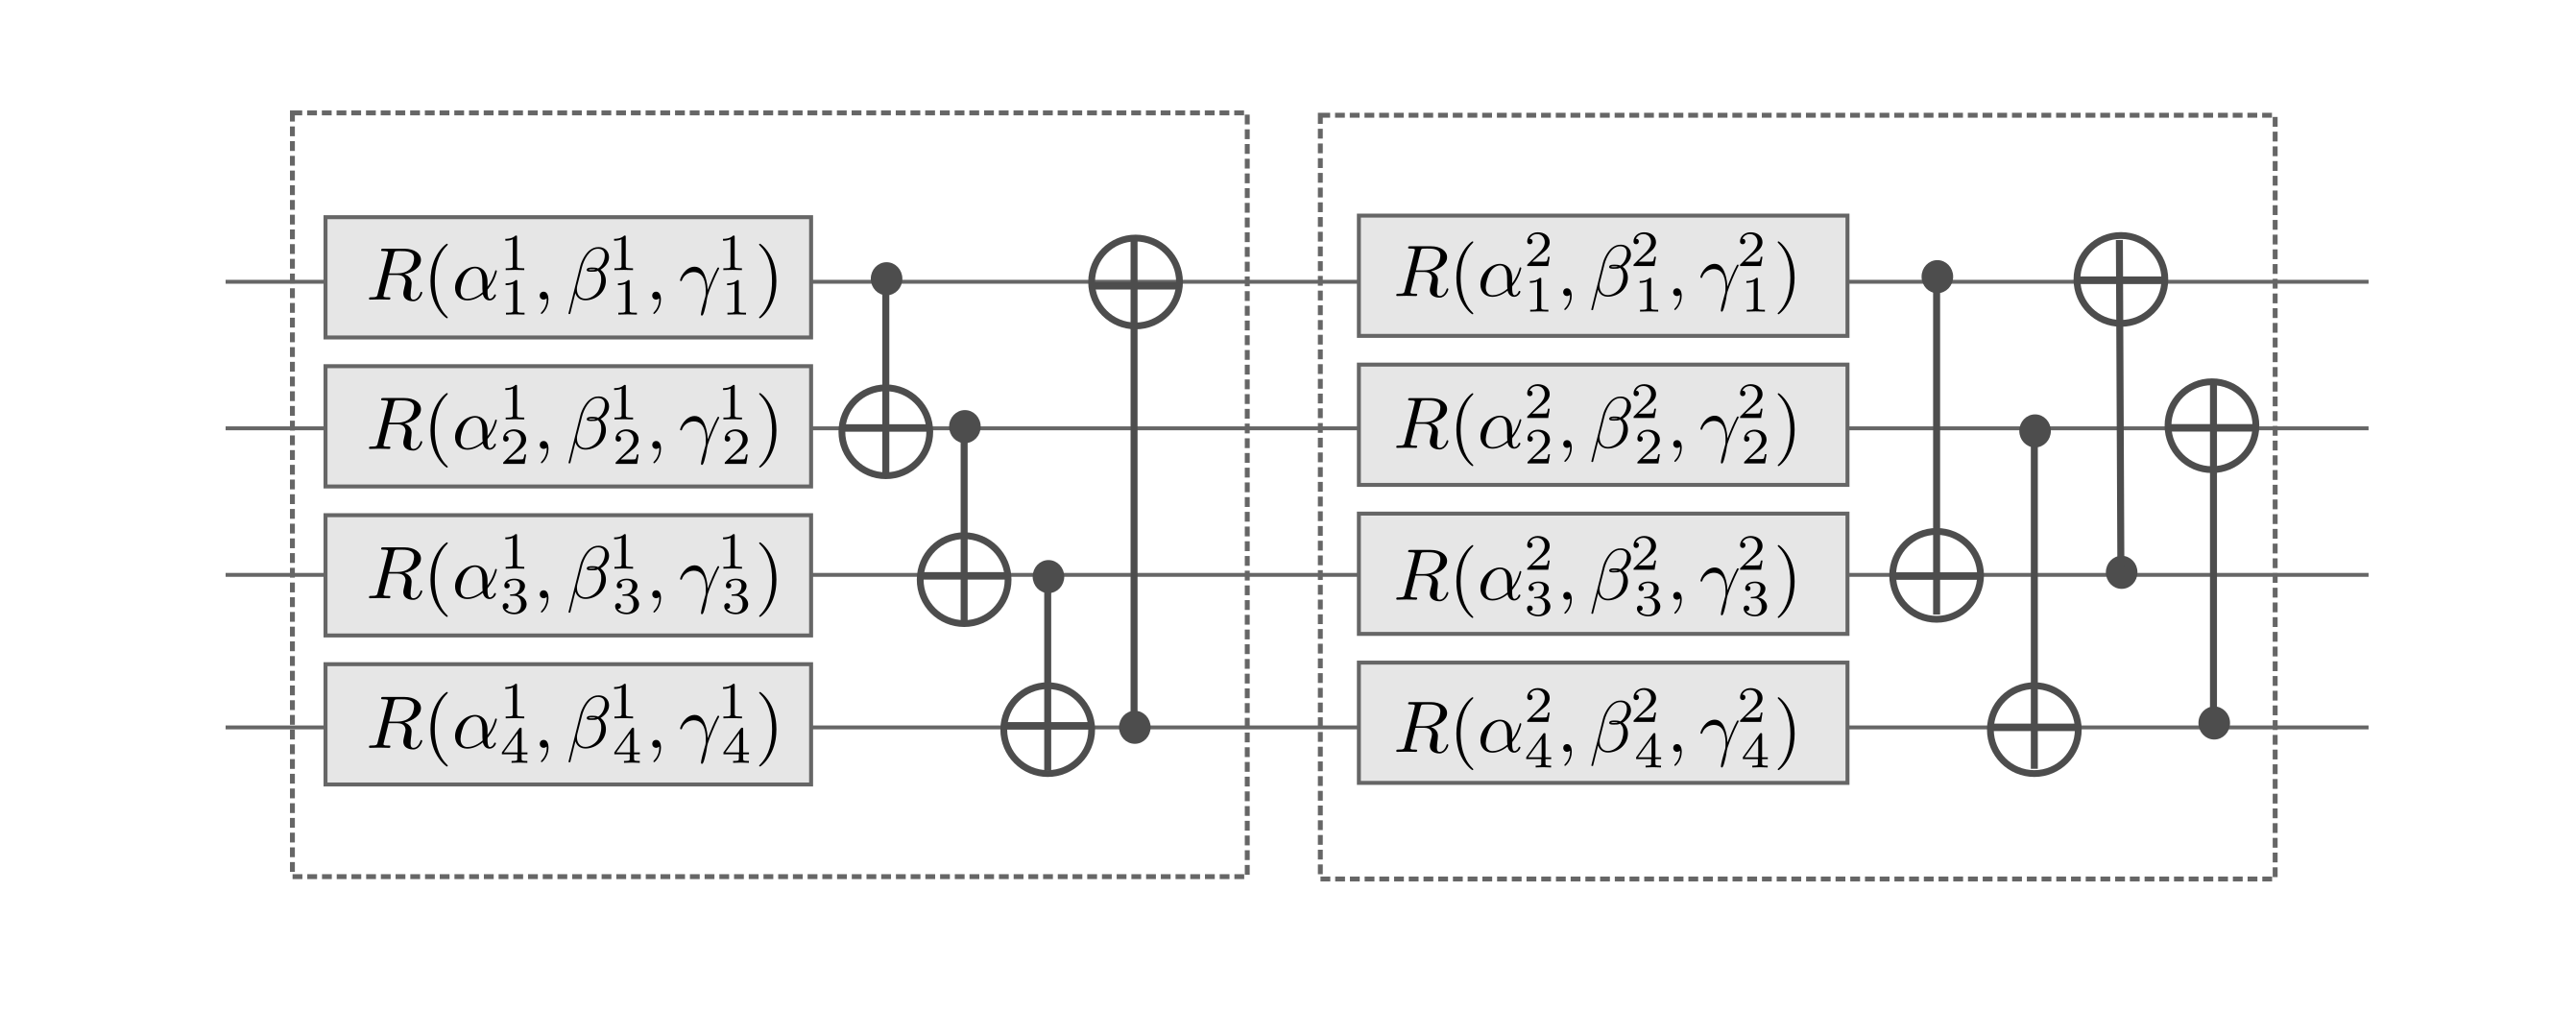
\includegraphics[width=0.8\linewidth]{figures/strongly_entangling_layers.png}
    \caption{Example of two 4-qubit strongly entangling layers (ranges \(r=1\) and \(r=2\), respectively) with rotations \(R\) and CNOTs as imprimitives, adapted from \textcite{pennylane_strongly_entangling_layers}.}
    \label{fig:layer-sec}
\end{figure}

The model output afterwards is computed from the expectation value of the Pauli-\(Z\)
observable measured on the first qubit. This expectation value is a scalar in
the interval \([-1,1]\), to which a trainable bias term \(b\) is added to obtain
the final score. 
The prediction rule is kept fixed across all CCC variants and the only systematic modification concerns the internal entangling structure of the variational circuit.

\section{Dequantized CCC Variants}

We consider controlled modifications of CCC designed to reduce or remove entanglement while preserving the rest of the architecture as far as possible. This follows the ablation perspective advocated by \textcite{bowles2024better}.

To this end, I introduce dequantized CCC variants that keep the same embedding, the same measurement rule, the same training pipeline, and the same overall role of the variational block, but replace the original ansatz by a custom controlled construction in which the amount of entanglement can be adjusted directly.

\subsection{Controlled Ansatz}

The modified ansatz is built layer by layer. Each layer first applies a trainable general single-qubit rotation on every qubit,
\[
\mathrm{Rot}(\alpha,\beta,\gamma),
\]
so the local trainable degrees of freedom are retained in all variants. The difference between variants lies only in how many of the candidate two-qubit couplings are actually activated.

Let $M$ be the total number of qubits. In layer $\ell$, the candidate entangling edges are defined by a cyclic offset
\[
r_\ell = (\ell \bmod (M-1)) + 1,
\]
which produces the ring-like edge set
\[
E_\ell = \{(i, i+r_\ell \bmod M) : i = 0,\dots,M-1\}.
\]
This means that successive layers cycle through different interaction ranges. From the candidate edge set, only a fraction is activated. If $\alpha \in [0,1]$ denotes the entanglement-control parameter, then the number of active entangling gates in layer $\ell$ is
\[
k_\ell = \mathrm{round}(\alpha |E_\ell|).
\]
 Here, $\mathrm{round}(\cdot)$ denotes rounding to the nearest integer. The active edges are chosen by seeded pseudorandom sampling, making the construction reproducible across runs while avoiding the same deterministic subset in every layer.

Operationally, $\alpha$ controls how much entangling structure is available to the circuit:
\begin{itemize}
  \item $\alpha = 0$ removes all two-qubit gates and yields a fully separable circuit,
  \item $0 < \alpha < 1$ produces partially entangling circuits, and
  \item $\alpha = 1$ refers to all the entangling gates activated, which is equivalent to \texttt{StronglyEntanglingLayers}.
\end{itemize}

\begin{figure}[H]
    \centering
    \setlength{\tabcolsep}{2pt}
    \renewcommand{\arraystretch}{1.0}

    \makebox[\textwidth][c]{%
    \begin{tabular}{cc}
        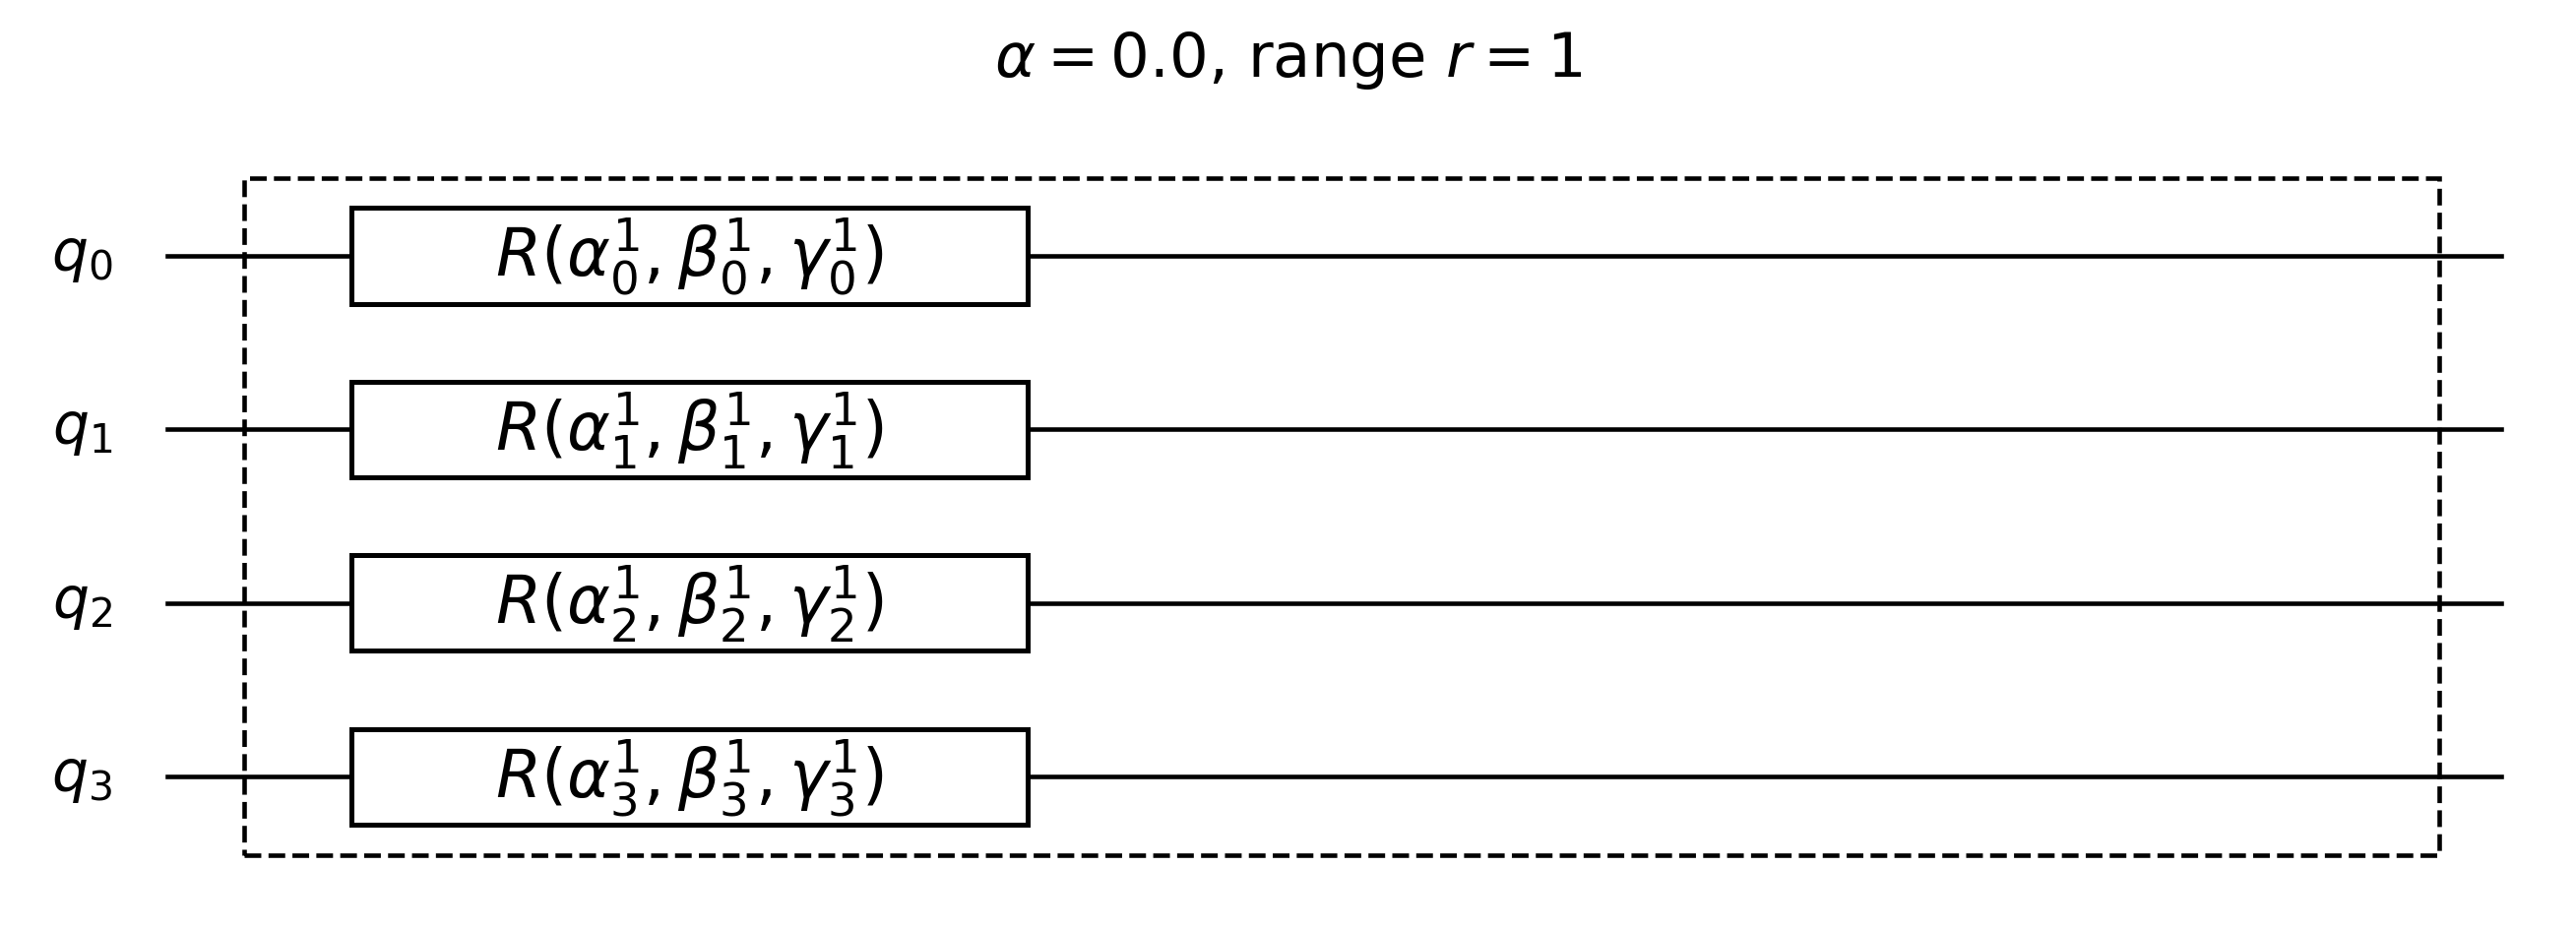
\includegraphics[width=0.53\textwidth,keepaspectratio]{figures/controlled_ccc/controlled_ccc_alpha_0p0_r1.png} &
        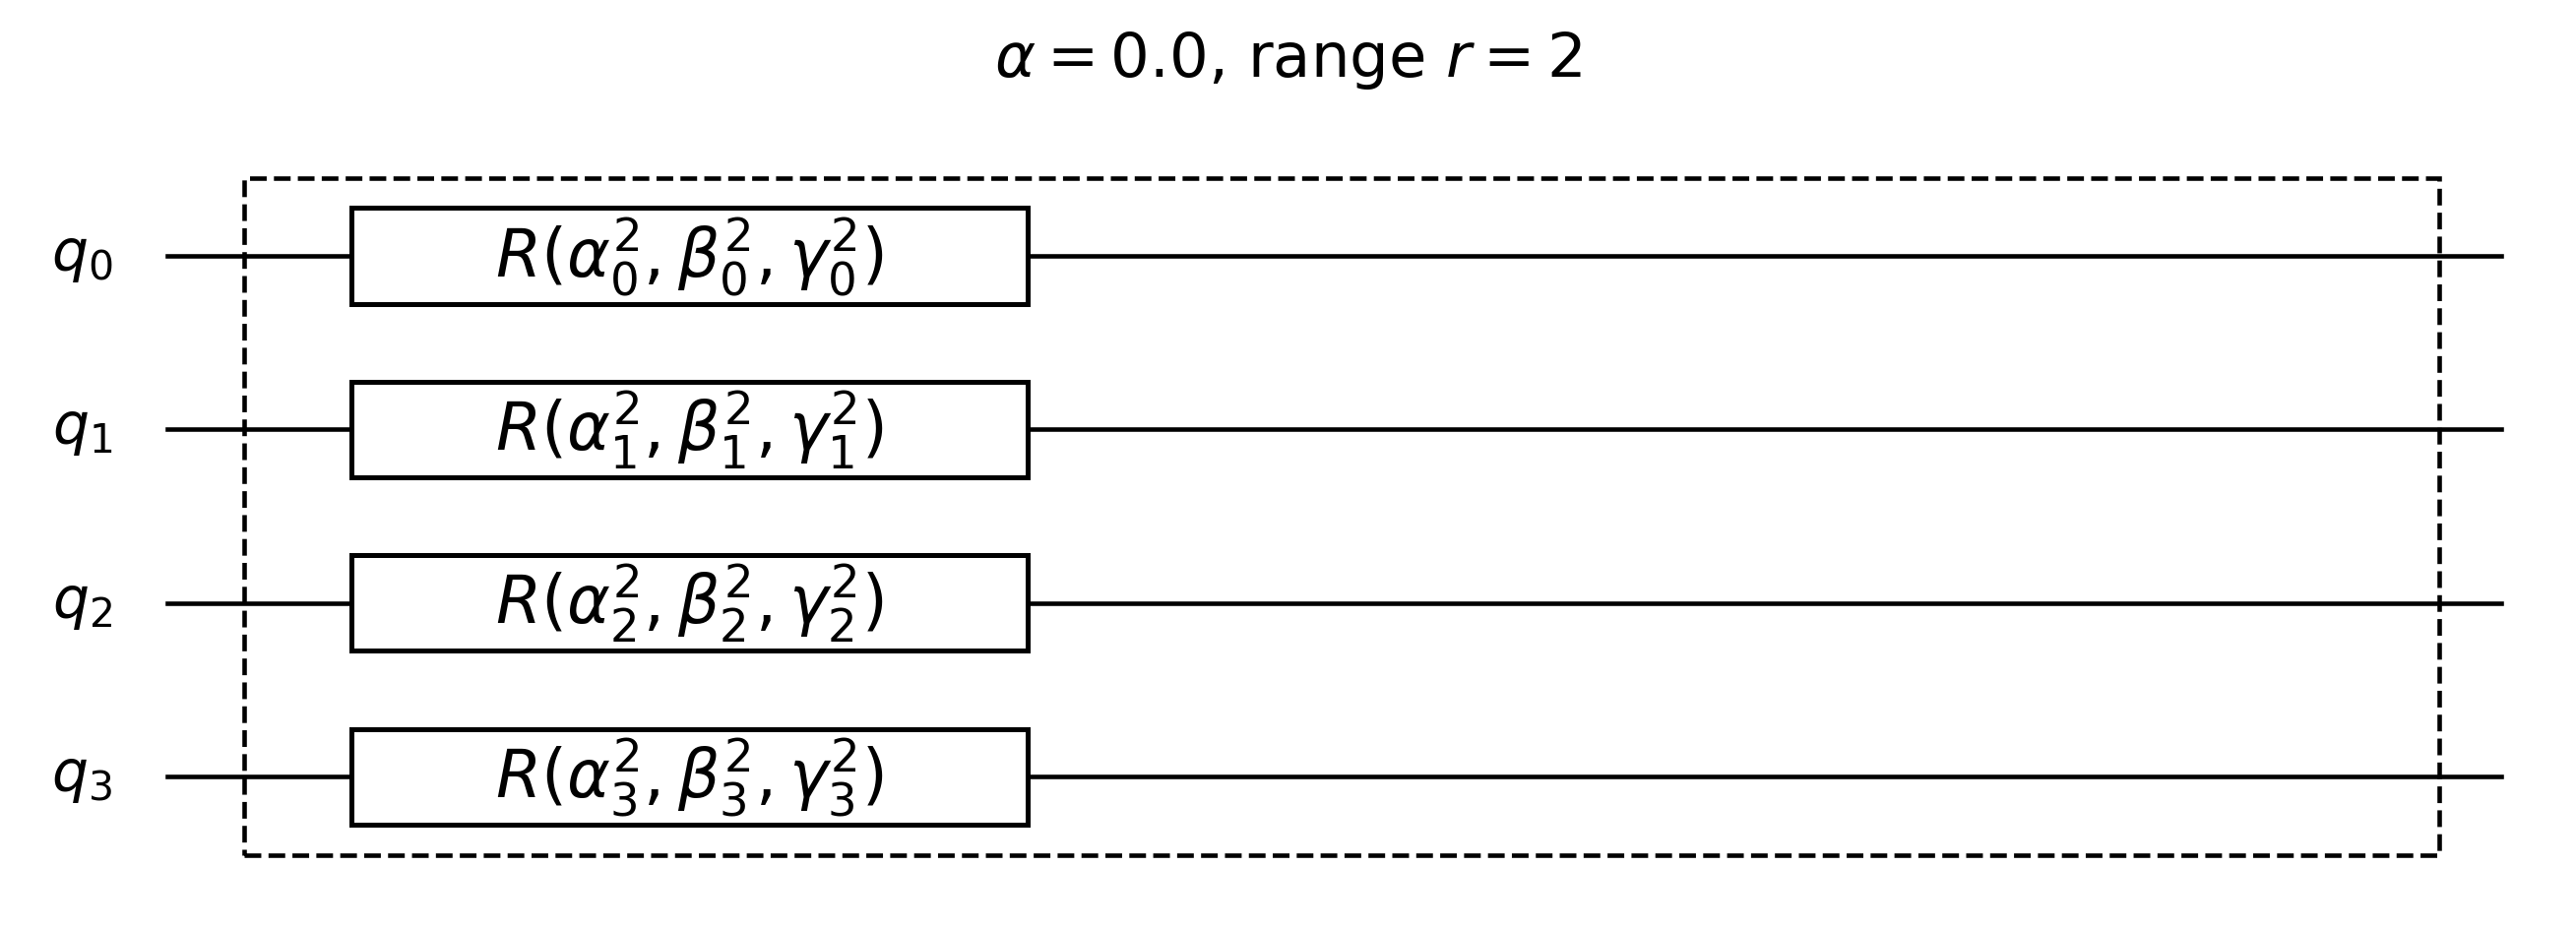
\includegraphics[width=0.53\textwidth,keepaspectratio]{figures/controlled_ccc/controlled_ccc_alpha_0p0_r2.png} \\[-0.2em]
        \multicolumn{2}{c}{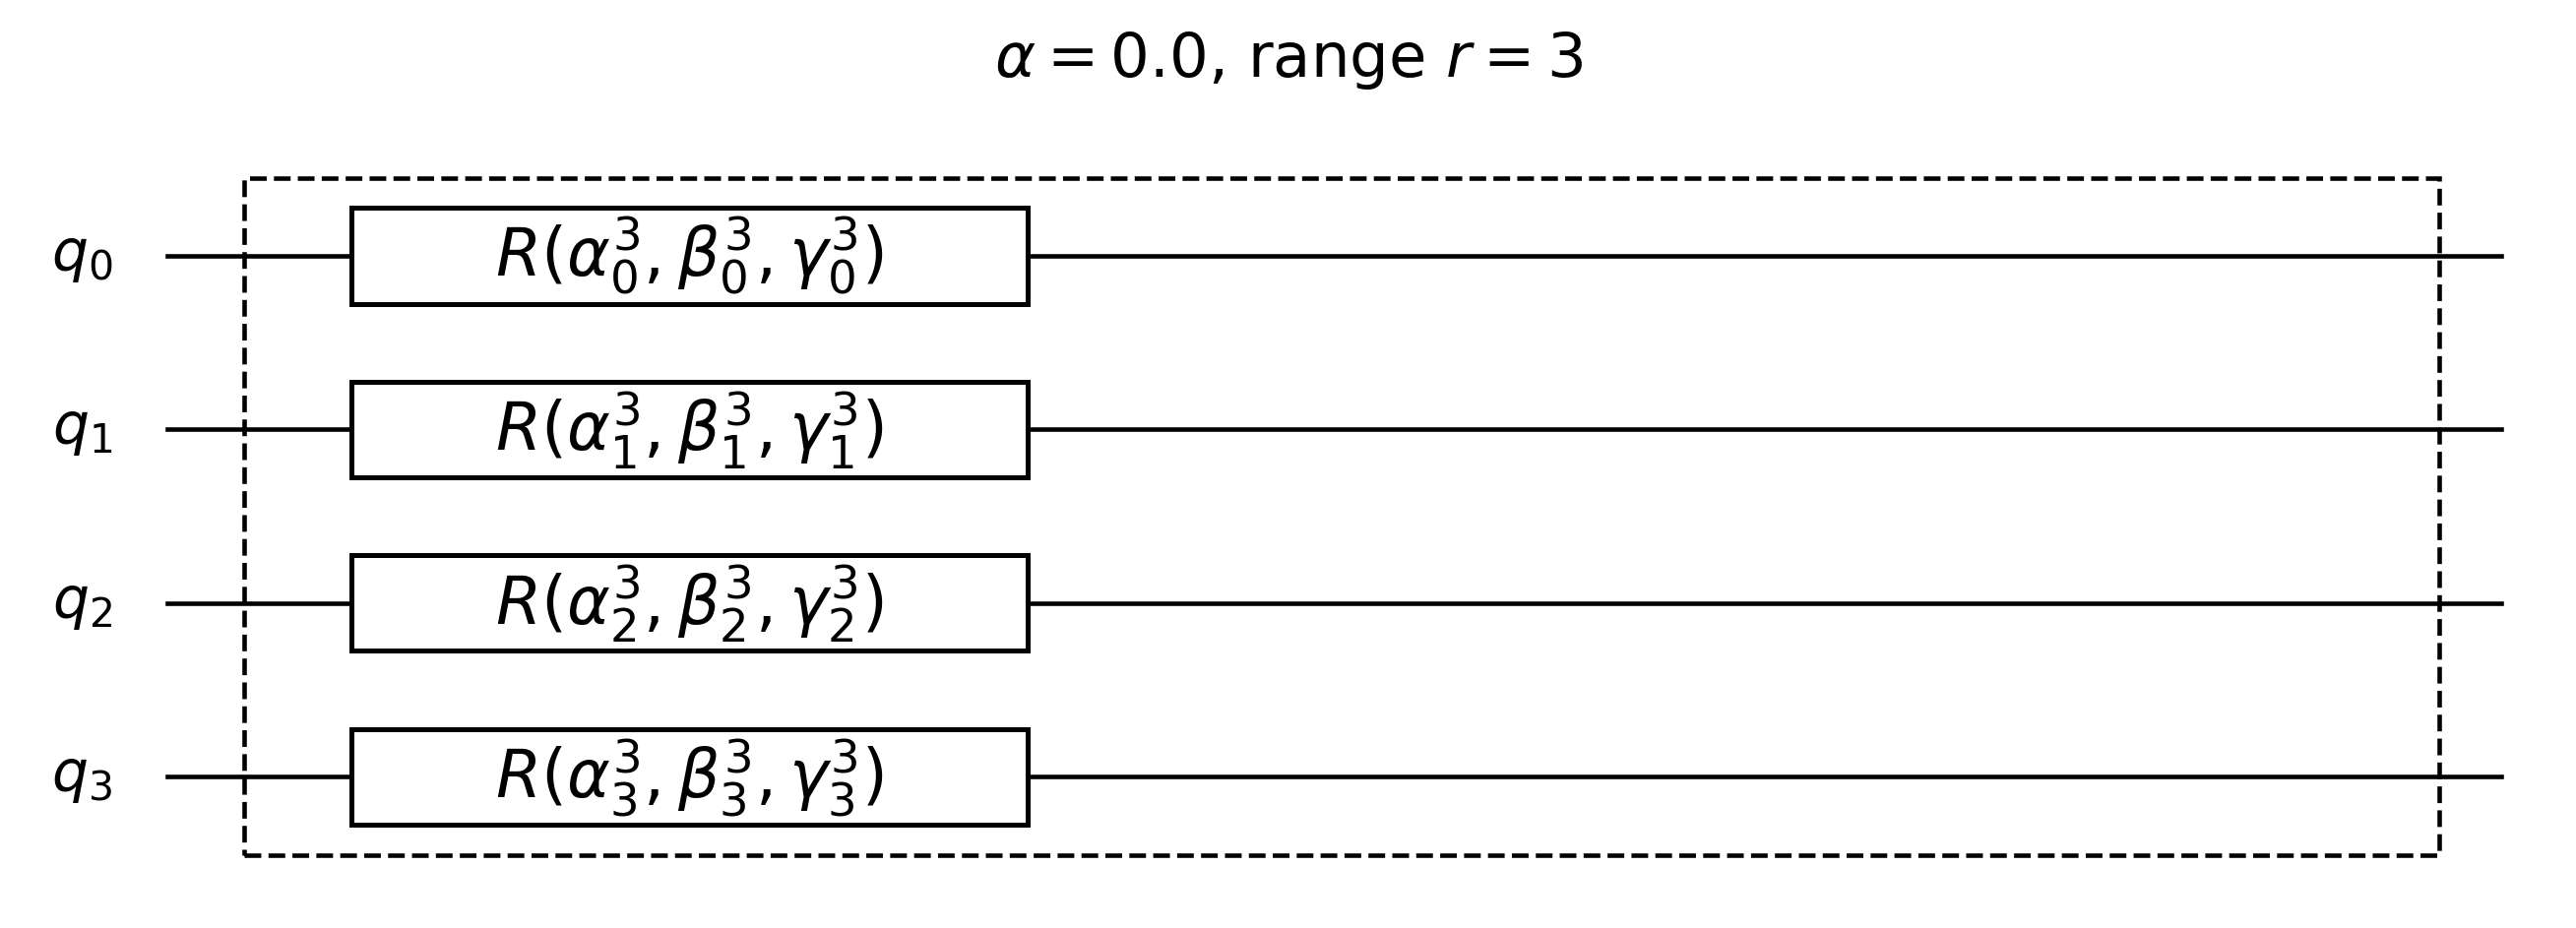
\includegraphics[width=0.53\textwidth,keepaspectratio]{figures/controlled_ccc/controlled_ccc_alpha_0p0_r3.png}} \\[0.2em]

        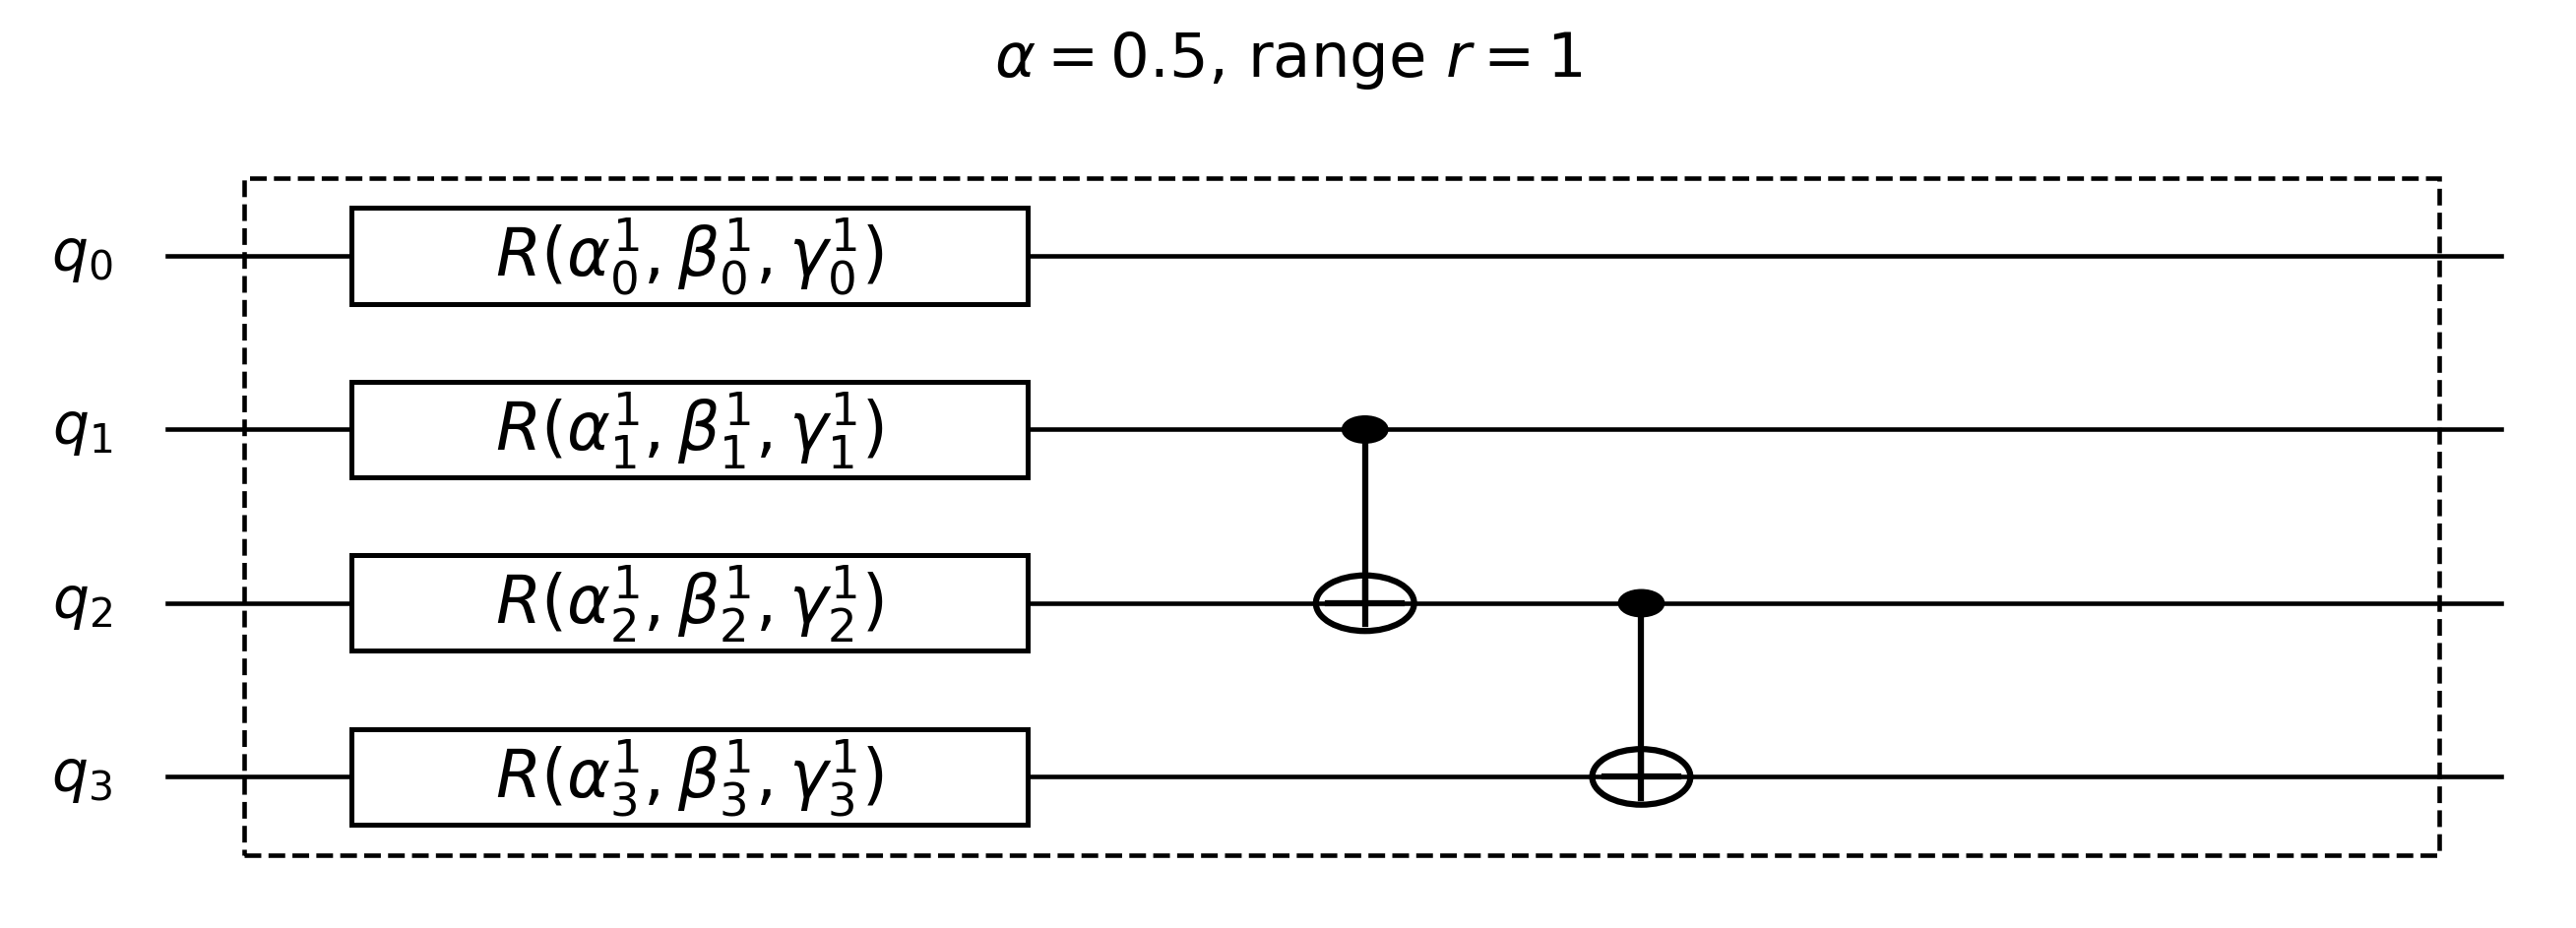
\includegraphics[width=0.53\textwidth,keepaspectratio]{figures/controlled_ccc/controlled_ccc_alpha_0p5_r1.png} &
        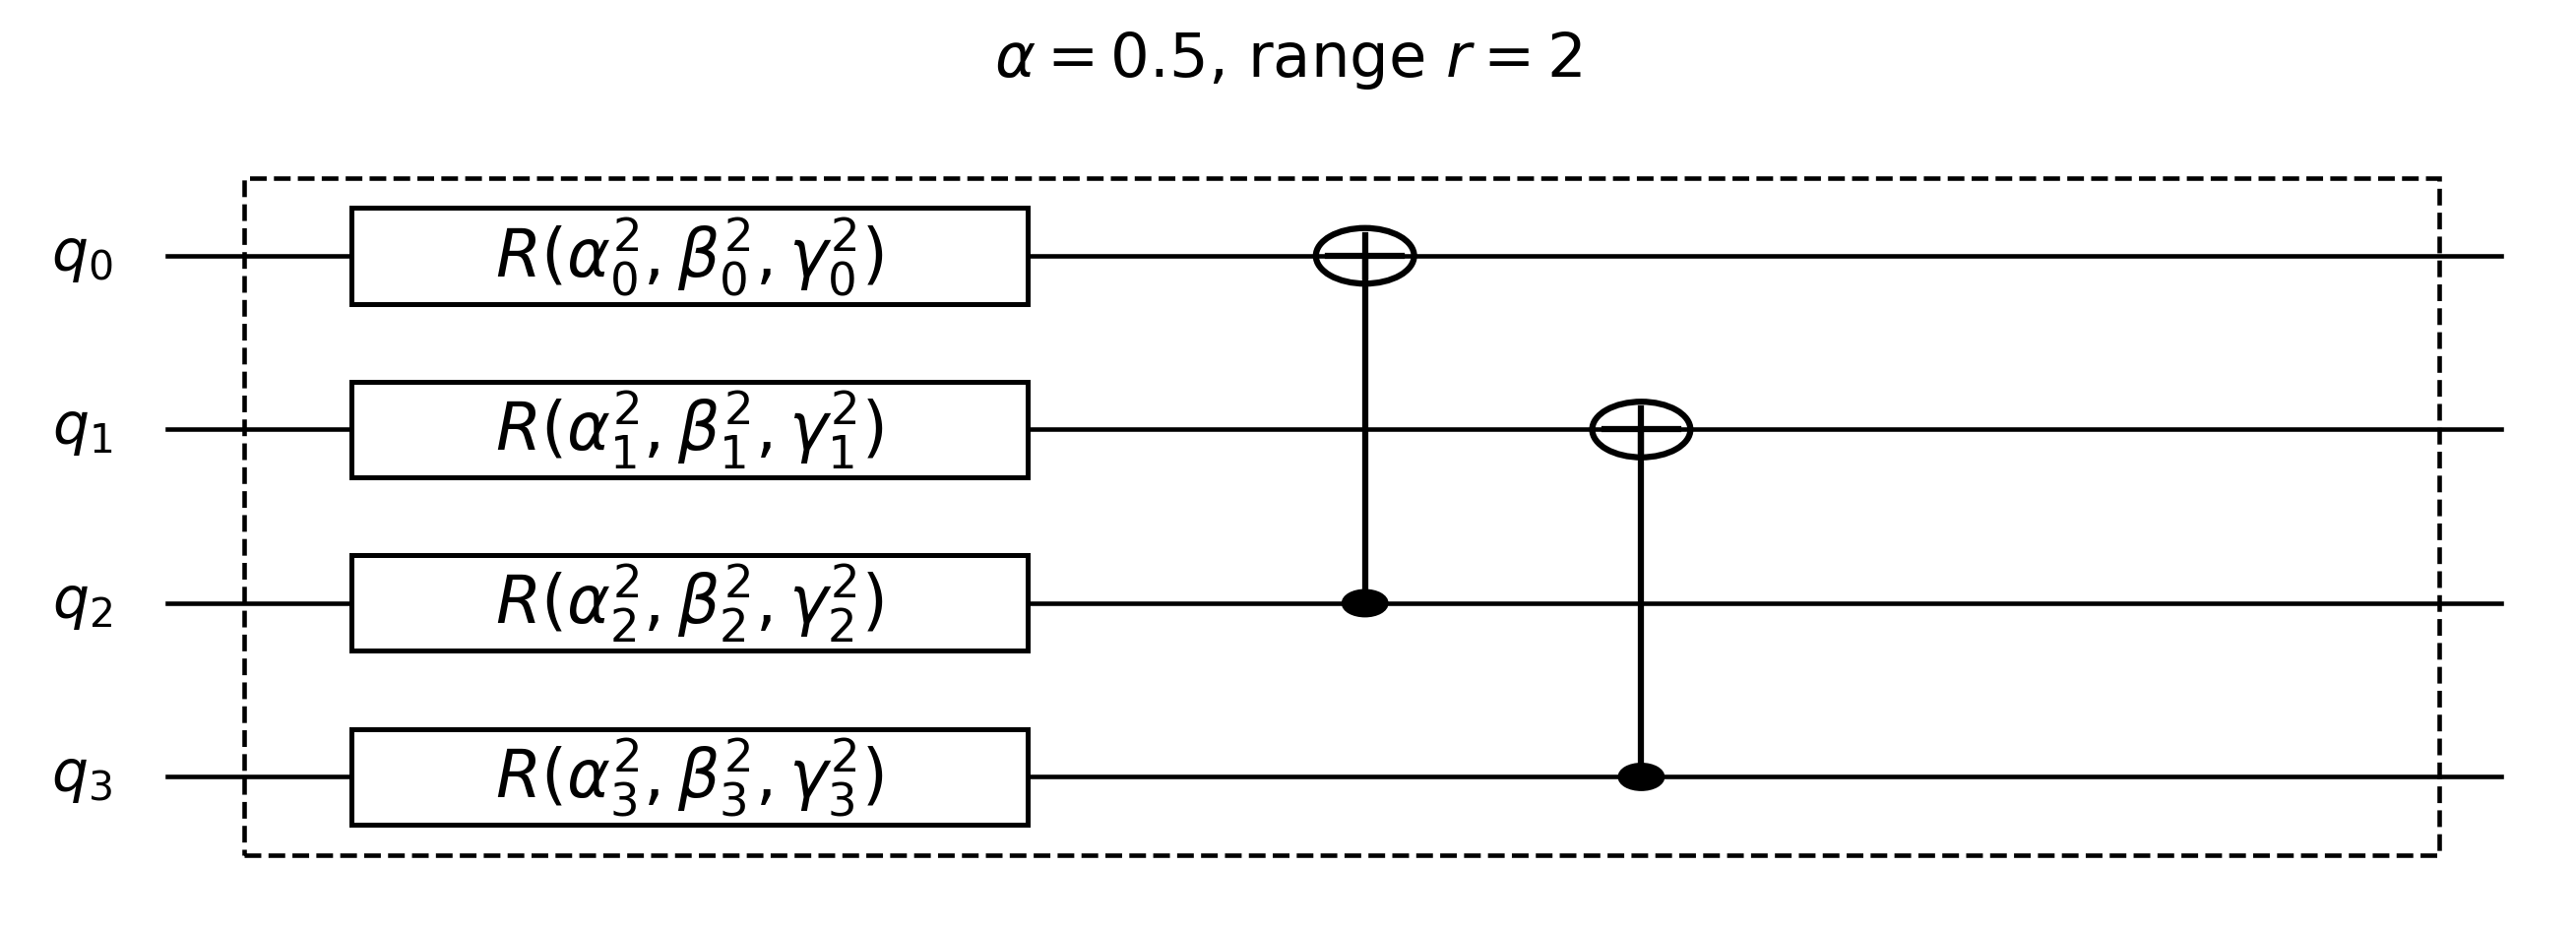
\includegraphics[width=0.53\textwidth,keepaspectratio]{figures/controlled_ccc/controlled_ccc_alpha_0p5_r2.png} \\[-0.2em]
        \multicolumn{2}{c}{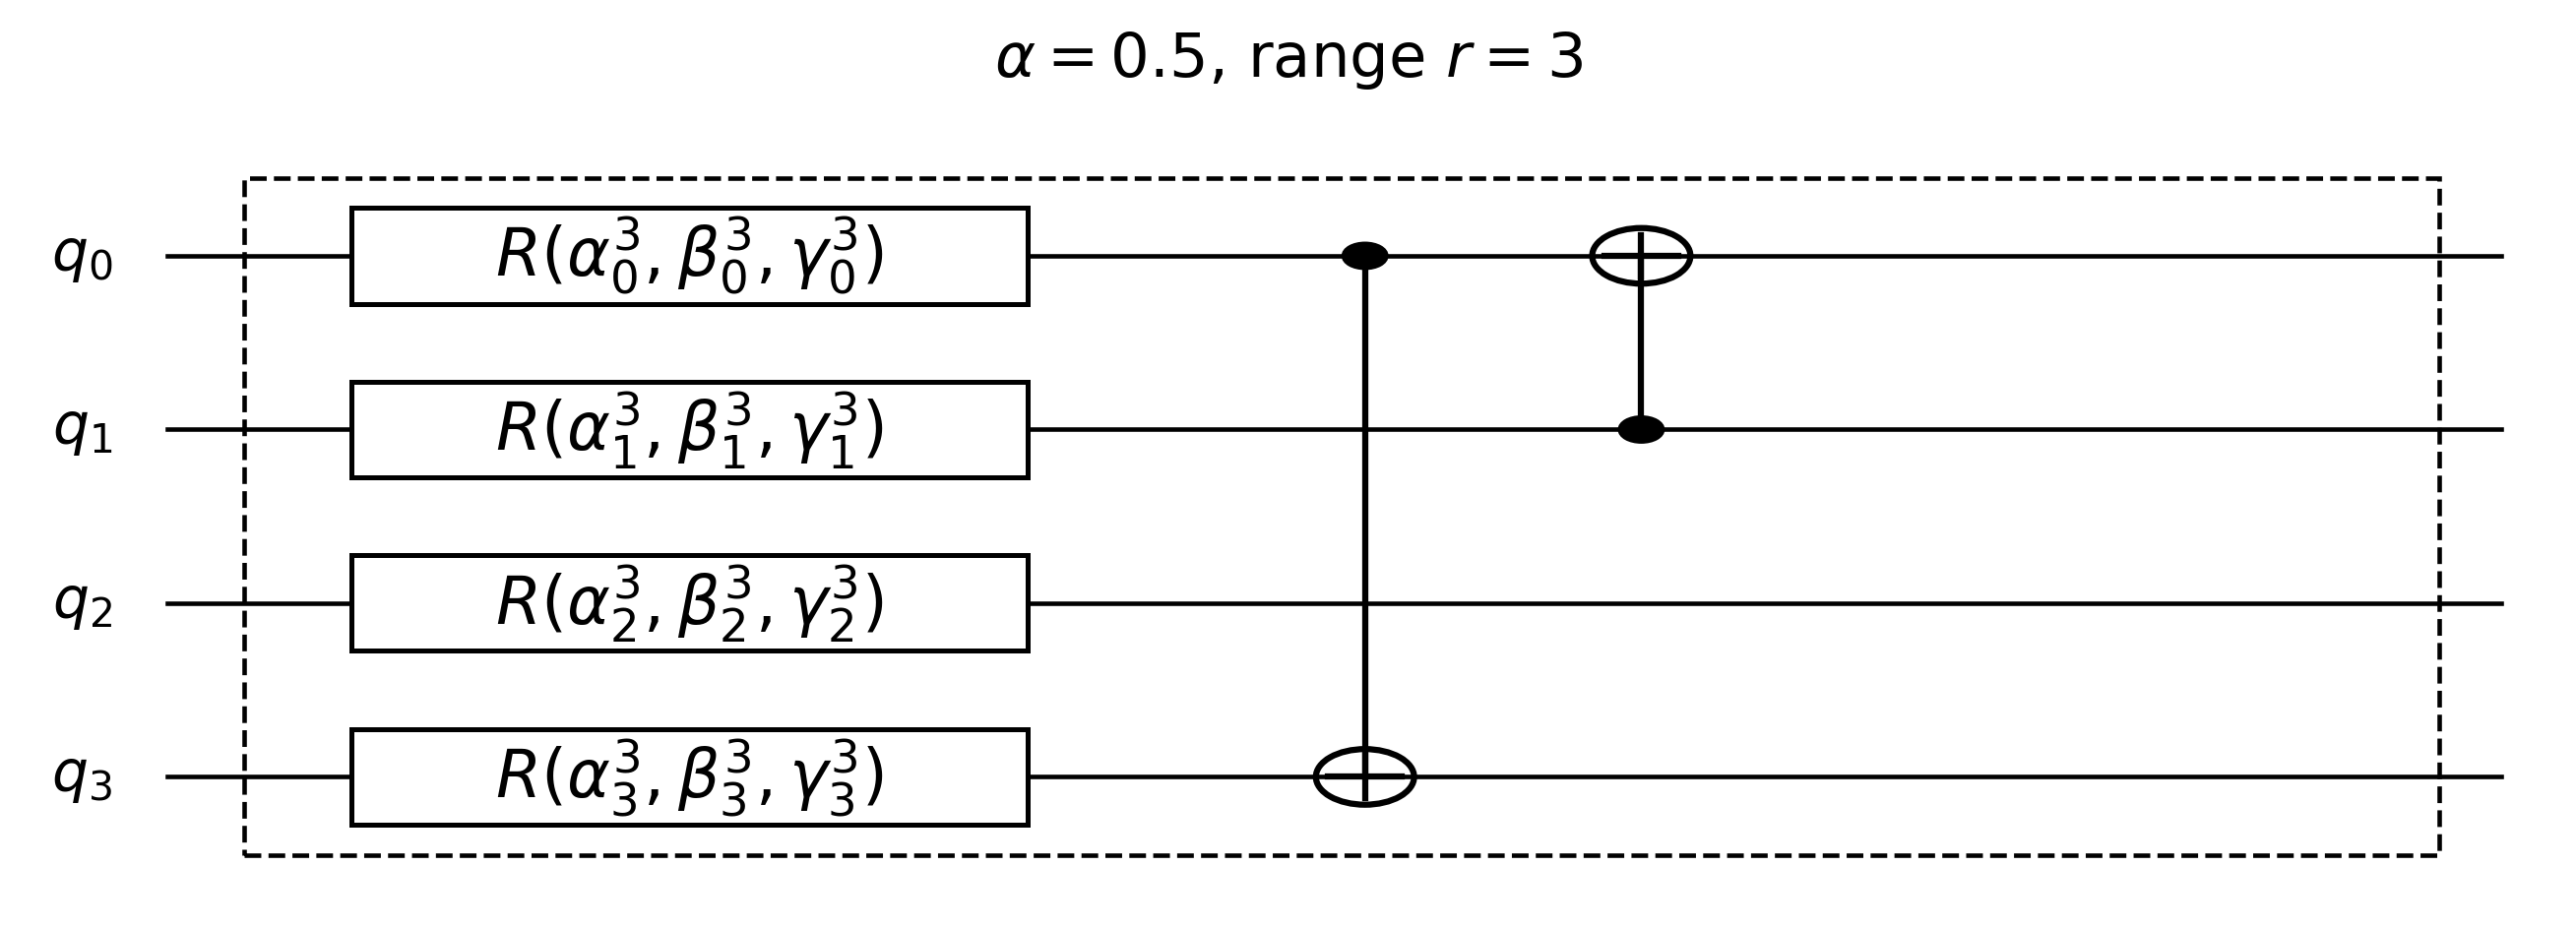
\includegraphics[width=0.53\textwidth,keepaspectratio]{figures/controlled_ccc/controlled_ccc_alpha_0p5_r3.png}} \\[0.2em]

        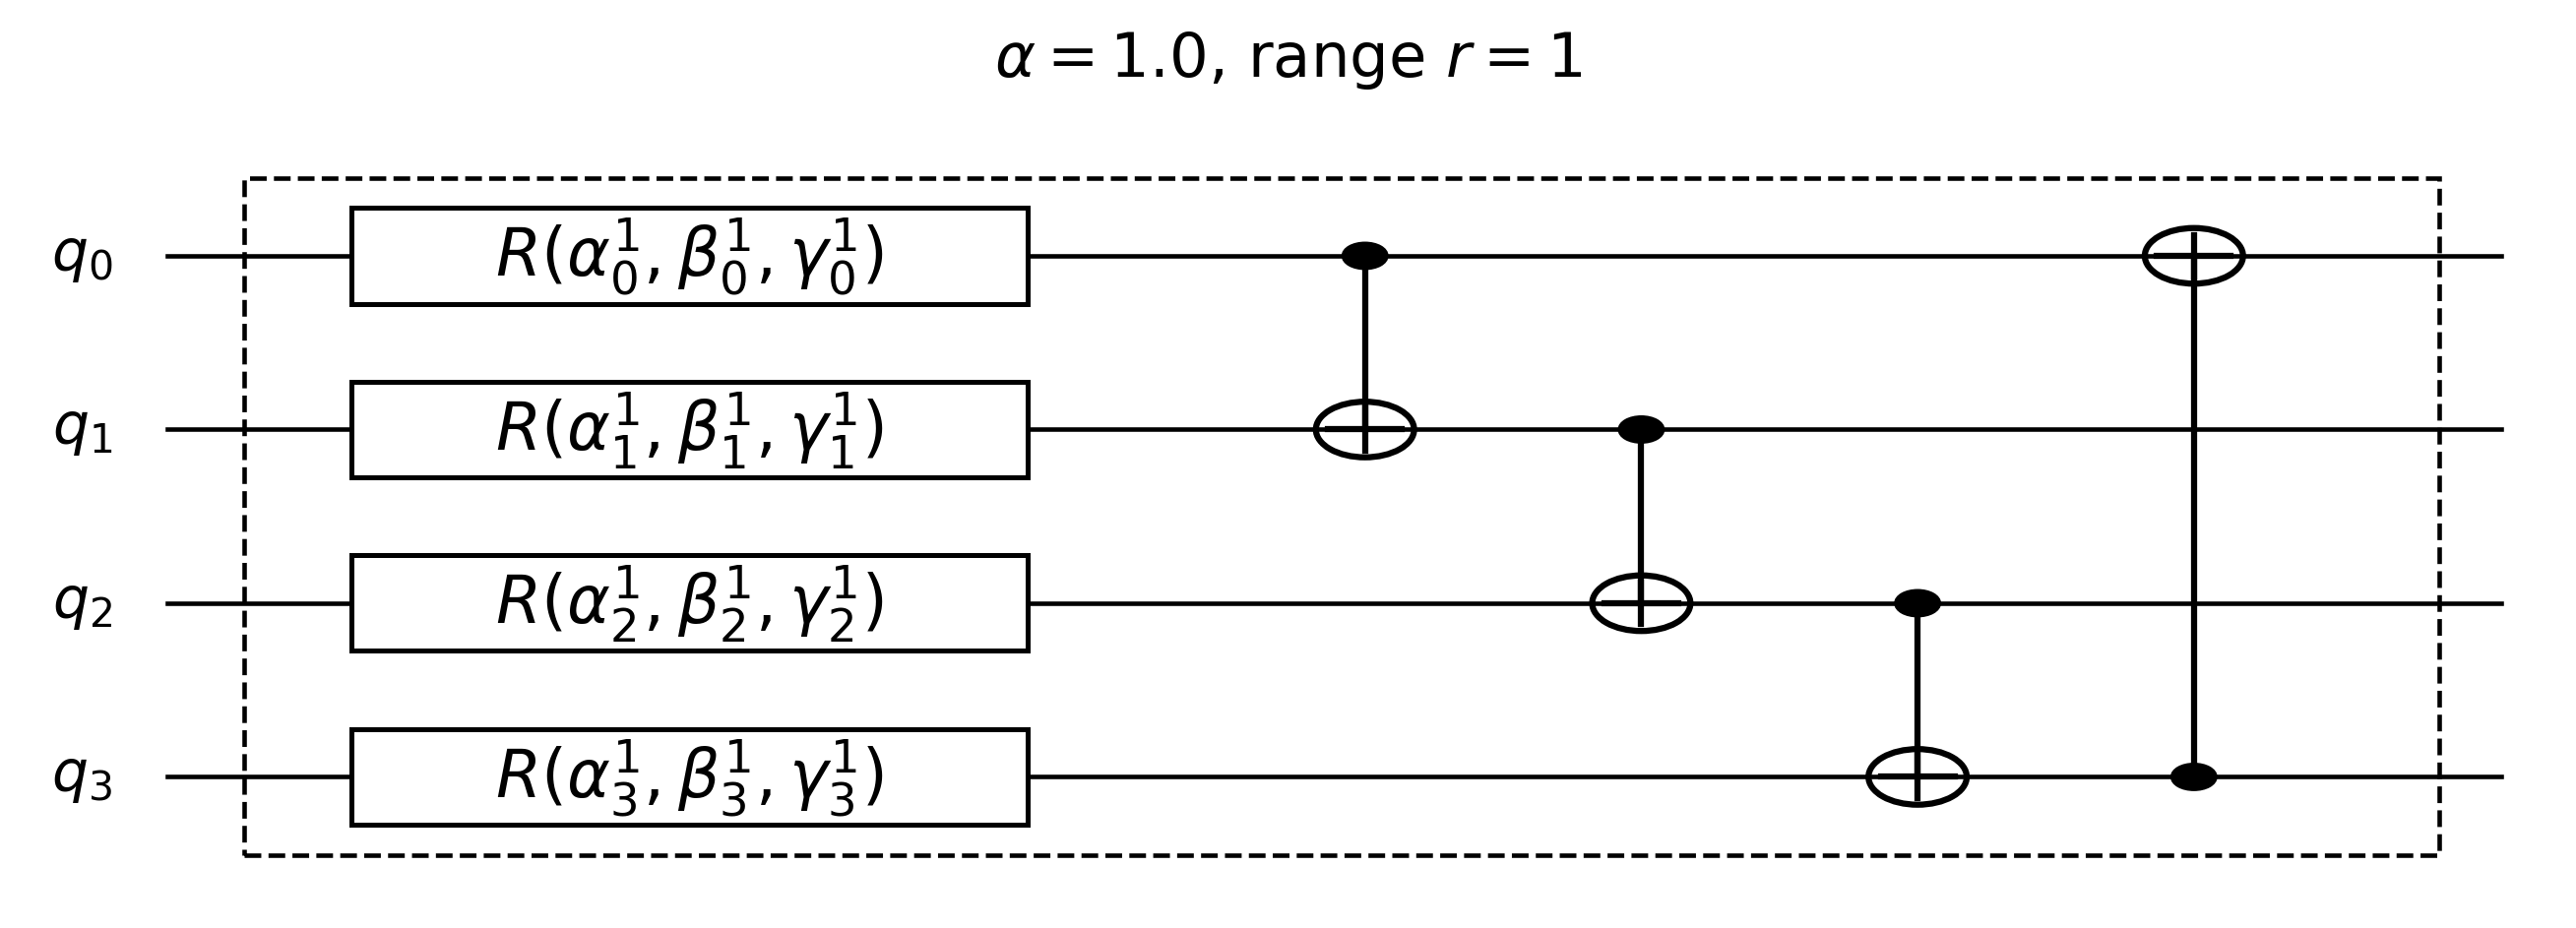
\includegraphics[width=0.53\textwidth,keepaspectratio]{figures/controlled_ccc/controlled_ccc_alpha_1p0_r1.png} &
        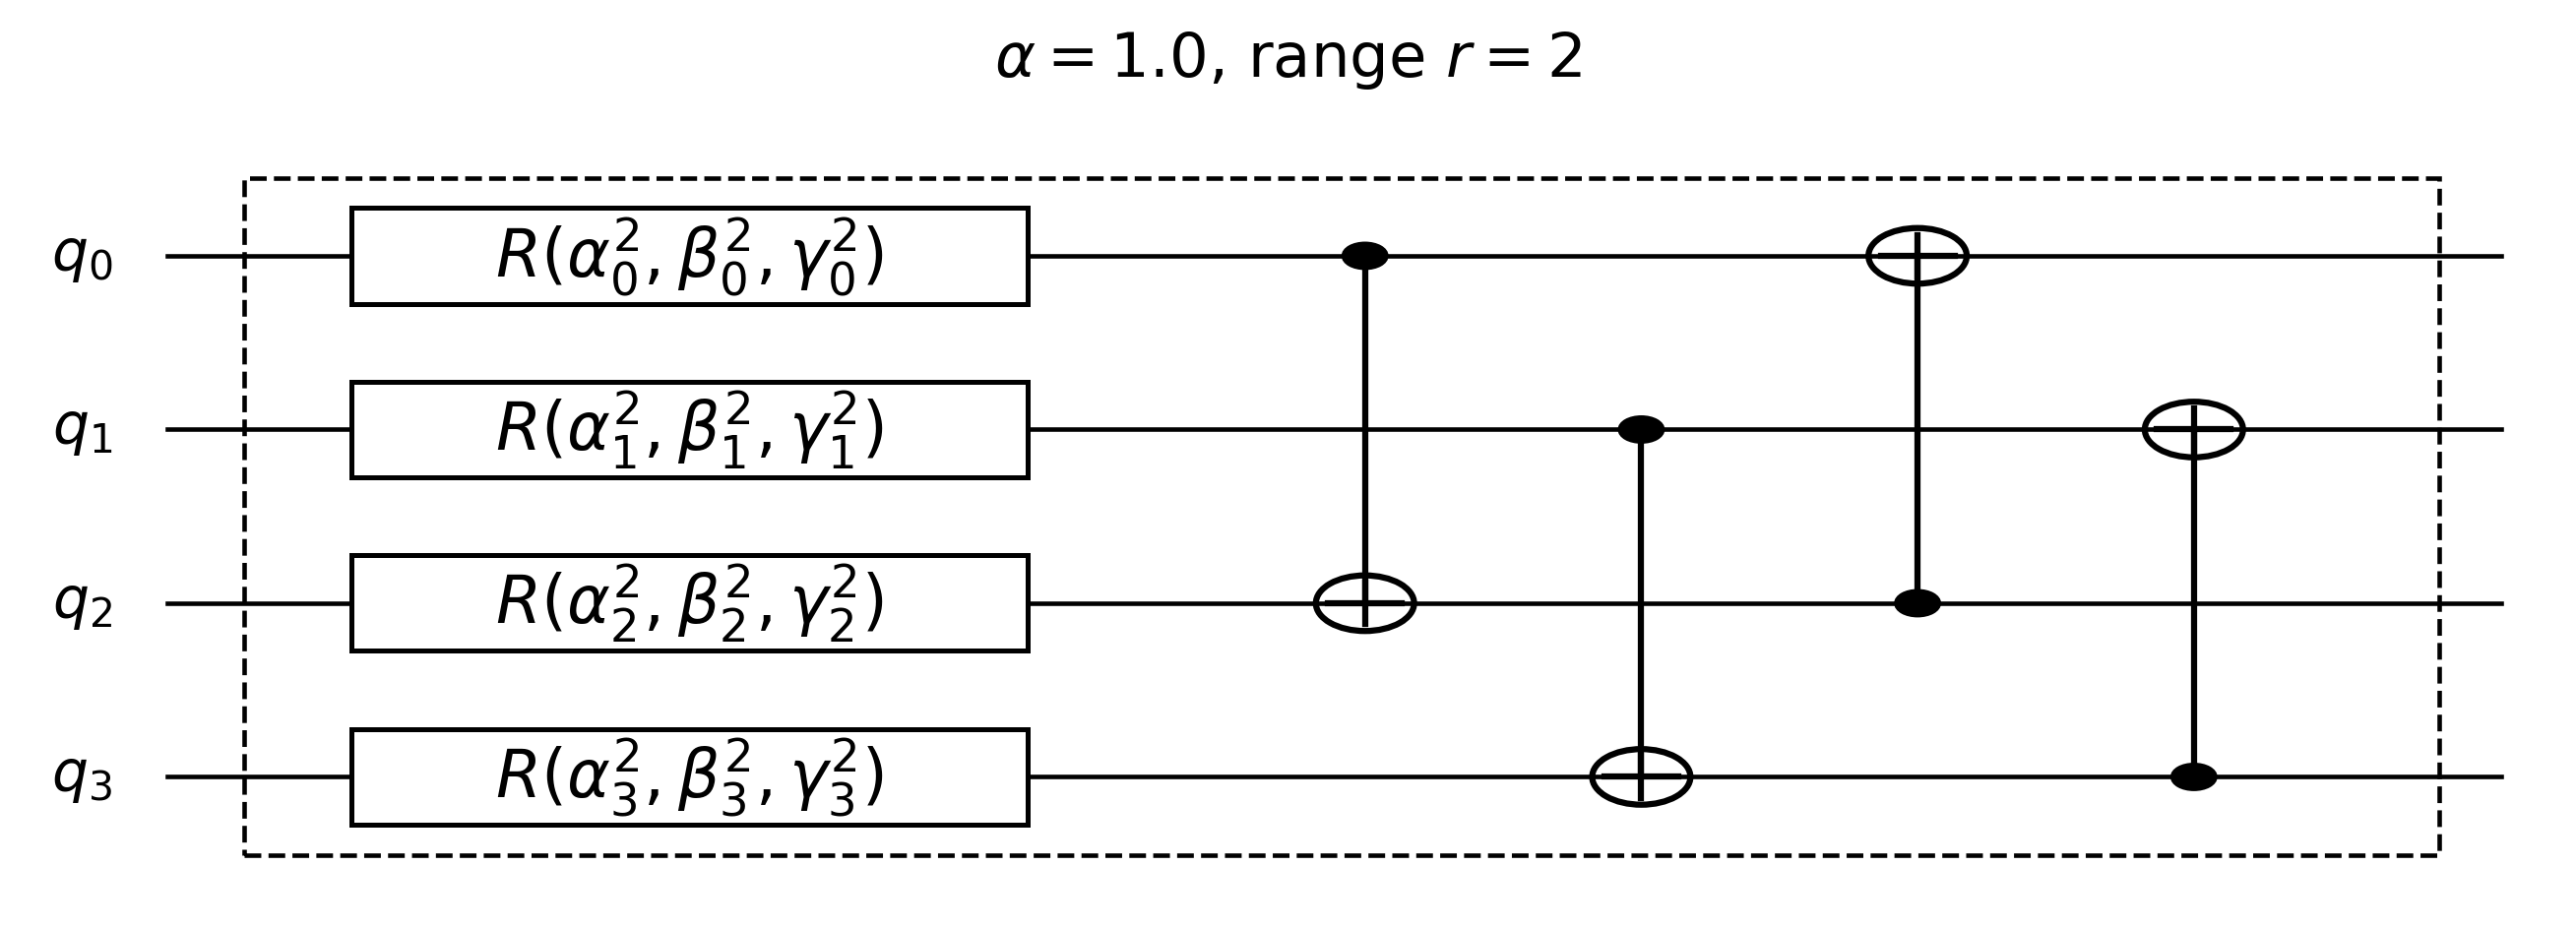
\includegraphics[width=0.53\textwidth,keepaspectratio]{figures/controlled_ccc/controlled_ccc_alpha_1p0_r2.png} \\[-0.2em]
        \multicolumn{2}{c}{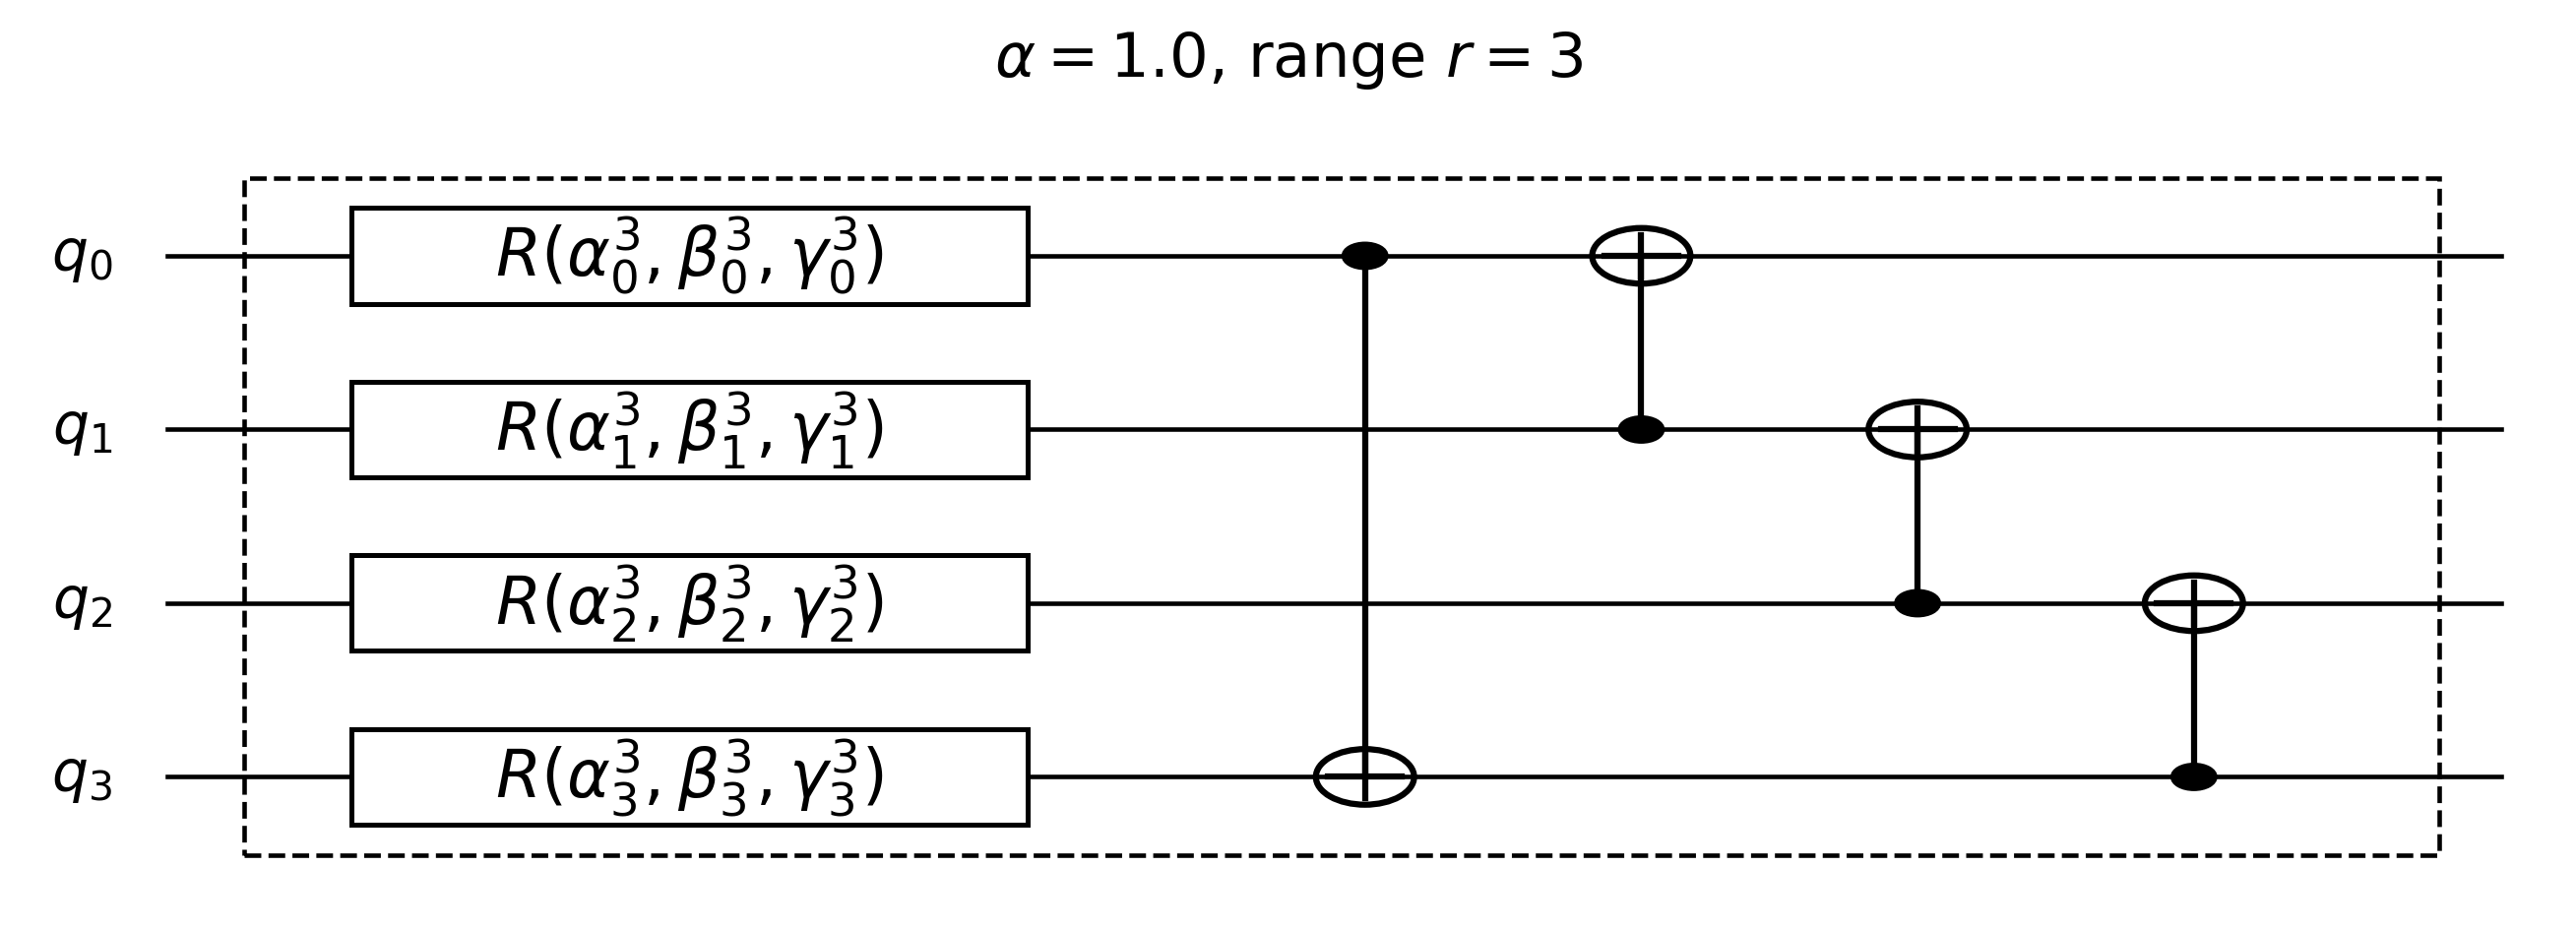
\includegraphics[width=0.53\textwidth,keepaspectratio]{figures/controlled_ccc/controlled_ccc_alpha_1p0_r3.png}}
    \end{tabular}%
    }

\caption{Example of the controlled CCC ansatz for \(M=4\) qubits and three interaction ranges \(r=1,2,3\). Each panel shows one layer consisting of local rotations \(R(\alpha_i^\ell,\beta_i^\ell,\gamma_i^\ell)\), followed by the active CNOT couplings selected by the entanglement-control parameter.}
    \label{fig:controlled-ccc-ansatz}
\end{figure}


\subsection{Separable and Half-Separable Variants}

Two dequantized variants are considered in this work.

The first is the \emph{separable} CCC. Here the entanglement-control parameter is set to $\alpha = 0$. As a result, no two-qubit gates are applied anywhere in the variational block. The circuit therefore remains fully local, and this constitutes the strongest dequantization step considered.

The second is the \emph{half-separable} CCC. Here the entanglement-control parameter is set to $\alpha = 0.5$, so that approximately half of the candidate two-qubit couplings in each layer remain active. This model occupies an intermediate position between the original entangling CCC and the fully separable version. It is methodologically useful because it allows us to test whether performance degrades gradually as entanglement is reduced, or whether most of the observed behavior can already be reproduced with only limited entangling structure. It uses a seeded random 50\% subset instead, which preserves reproducibility while avoiding this ordering bias.

The implementation of this controlled ansatz is shown in
Listing~\ref{lst:controlled-ansatz-relevant}, which is a modified version from \ref{lst:strongly-entangling-relevant}.
\begin{lstlisting}[
    style=pythonstyle,
    caption={Relevant logic of PennyLane's \texttt{StronglyEntanglingLayers} template~\parencite{pennylane_strongly_entangling_layers}.},
    label={lst:strongly-entangling-relevant}
]
for l in range(n_layers):

    # Single-qubit rotation on every qubit
    for i in range(len(wires)):
        op_list.append(
            Rot(
                weights[..., l, i, 0],
                weights[..., l, i, 1],
                weights[..., l, i, 2],
                wires=wires[i],
            )
        )

    if len(wires) > 1:
        # Candidate entangling edges for range ranges[l]
        for i in range(len(wires)):
            act_on = wires.subset(
                [i, i + ranges[l]],
                periodic_boundary=True,
            )

            # All candidate edges are active
            op_list.append(imprimitive(wires=act_on))
\end{lstlisting}

\begin{lstlisting}[
    style=pythonstyle,
    caption={Relevant controlled-ansatz logic implemented in \texttt{src/qml\_benchmarks/models/circuit\_centric.py}.},
    label={lst:controlled-ansatz-relevant}
]
for l in range(self.n_layers):

    # Single-qubit rotation on every qubit
    for i in range(M):
        qml.Rot(
            weights[l, i, 0],
            weights[l, i, 1],
            weights[l, i, 2],
            wires=i,
        )

    if M > 1:
        # Interaction range for layer l
        r = (l % (M - 1)) + 1

        # Ring-like candidate entangling edge set
        edges = [(i, (i + r) % M) for i in range(M)]

        # Entanglement-control parameter alpha
        # alpha = self.entanglement_level
        k = int(round(self.entanglement_level * len(edges)))

        if k > 0:
            rng = np.random.default_rng(
                self.random_state + 1000 * l
            )

            # Active entangling edges
            idx = rng.choice(len(edges), size=k, replace=False)
            idx.sort()

            for j in idx:
                a, b = edges[j]
                gate(wires=[a, b])
\end{lstlisting}

The concrete half-separable and fully separable CCC variants are obtained through wrapper classes that use the same controlled ansatz but fix \texttt{entanglement\_level} to \(0.5\) and \(0.0\), respectively, as shown below.
\refstepcounter{lstlisting}
\noindent\begin{minipage}{\textwidth}
\centering

\begin{minipage}{0.48\textwidth}
\begin{lstlisting}[style=pythonstyle, basicstyle=\ttfamily\scriptsize, numbers=none]
class HalfSeparable(CircuitCentricClassifier):
    def __init__(self, ...):
        super().__init__(
            ansatz_type="controlled",
            entanglement_level=0.5, ...
        )
\end{lstlisting}
\end{minipage}
\hfill
\begin{minipage}{0.48\textwidth}
\begin{lstlisting}[style=pythonstyle, basicstyle=\ttfamily\scriptsize, numbers=none]
class Separable(CircuitCentricClassifier):
    def __init__(self, ...):
        super().__init__(
            ansatz_type="controlled",
            entanglement_level=0.0, ...
        )
\end{lstlisting}
\end{minipage}

\label{lst:ccc-wrapper-minimal}
\par\smallskip
{\small Listing \thelstlisting: Wrappers for half-separable and fully separable CCC variants.\par}
\end{minipage}

\section{IQP Kernel Classifier}

The second quantum model family studied in this thesis is the IQP kernel classifier, based on the \texttt{IQPKernelClassifier} already present in the benchmark codebase. This family is included so that the entanglement-ablation question can be asked not only for a variational classifier, but also for a quantum-kernel model.

The IQP kernel model differs conceptually from CCC in an important way. CCC is a variational classifier with trainable circuit parameters and a measurement-based prediction rule. By contrast, the IQP-kernel model uses a fixed feature map to define a kernel
\[
    k(x,x') = |\langle 0|U(x')^{\dagger}U(x)|0\rangle|^2,
\]
which is then passed to a classical support-vector machine with a precomputed kernel matrix. In other words, the quantum circuit defines the feature space, while the final classifier is a classical SVM.

In the implementation used here, the single-qubit part of the IQP feature map is kept fixed across all variants, and only the ZZ entangling pattern is changed. The hyperparameter interface is also kept aligned across variants, in particular the number of IQP repeats and the SVM regularisation parameter.

\subsection{IQP Kernel Variants}

Three IQP-kernel variants are considered.

The first is the original \texttt{IQPKernelClassifier}, which uses the standard IQP-style feature map with all ZZ couplings present in each repeat of the embedding.

The second is \texttt{IQPKernelClassifierSeparable}. This variant keeps the same single-qubit IQP encoding but removes all ZZ couplings. It is therefore the direct no-entanglement ablation for the IQP feature map.

The third is \texttt{IQPKernelClassifierHalfSeparable}. This variant again keeps the same single-qubit IQP encoding, but for each repeat it retains only a seeded random 50\% subset of the full ZZ edge set. As in the CCC case, the intention is to test whether reducing entangler density causes a gradual loss relative to the full model, or whether much of the kernel's behavior can already be recovered with a sparse entangling pattern.

These IQP-kernel variants are methodologically useful because they allow the entanglement question to be posed in a different QML model class. In CCC, entanglement appears inside a trainable variational ansatz. In the IQP-kernel model, by contrast, the entangling ZZ structure is part of the fixed feature map itself. Comparing both families therefore helps separate claims about entanglement in a particular ansatz from claims about entanglement in a broader QML pipeline.

\section{Training Procedure}

All model variants are trained within the same benchmark pipeline. This includes the same dataset generation, the same train-test protocol, the same hyperparameter-search infrastructure, and the same result logging format. The purpose of this uniform setup is to ensure that the comparison between CCC and its dequantized variants is an ablation study of model structure rather than a comparison between different experimental conditions.

For CCC, the implementations are trained as binary classifiers with labels in $\{-1,+1\}$. The model parameters consist of the variational circuit parameters together with the scalar bias term. Hyperparameters such as the number of input copies, the number of variational layers and learning rate are selected through the same search procedure used by the benchmark framework. This point matters because, as emphasized by \textcite{bowles2024better}, hyperparameter tuning can strongly affect benchmark outcomes in QML.

For the IQP-kernel family, the training flow is different but the benchmarking philosophy is the same. The quantum circuit is used to construct kernel matrices, and classification is then performed by a classical SVM backend. The main hyperparameters are the number of IQP repeats and the SVM regularisation parameter.
\section{Evaluation}

Model performance is evaluated primarily through test accuracy on the benchmark tasks. The central object of interest is the relative ranking of the original and dequantized CCC variants across datasets and benchmark settings. The experiments therefore examine not only absolute scores, but also whether removing entanglement changes the ordering of models across tasks of different difficulty.

All reported results come from the benchmark framework described in this chapter. Train accuracy is used only as a secondary diagnostic to assess whether changes in test performance are associated with changes in fitting capacity or with possible overfitting.

\section{Reproducibility}
All experiments were conducted within a modified benchmark setup based on the \texttt{qml\_benchmarks} repository. The exact codebase used in this thesis is available at \url{https://github.com/Mauricio-GutierrezL/Thesis}. This repository provided the common experimental pipeline for dataset handling, model training, hyperparameter selection, and final evaluation. The overall benchmarking methodology follows the framework discussed by \citet{bowles2024better}. The computational environment was based on Python 3.9.21 and used PennyLane 0.38.0 together with JAX, with 64-bit precision enabled via \path{jax.config.update("jax_enable_x64", True)}. Additional core dependencies included scikit-learn, NumPy, and matplotlib. The modified implementations of the Circuit-Centric Classifier variants introduced in this thesis are located in \path{src/qml_benchmarks/models/circuit_centric.py}. Benchmark datasets were stored under \path{thesis/datasets_tests/}, while experiment outputs and aggregated results were written to \path{thesis/my_results/}.

All runs were executed on the RWTH Aachen CLAIX HPC cluster using CPU-only jobs scheduled through Slurm. Hyperparameter optimization was performed with \texttt{GridSearchCV} using five-fold cross-validation, and the same train/test evaluation pipeline was applied uniformly across all compared models in order to ensure methodological consistency.

Benchmark datasets were generated with the utility script \path{thesis/generate_paper_benchmarks.py}, built on top of the data-generation functions in \path{src/qml_benchmarks/data/}. The benchmark-specific parameter choices in this script follow the original benchmark-generation setup from \path{paper/benchmarks/}. Dataset generation used fixed seeds per benchmark family, including \texttt{42} for linearly separable and MNIST-PCA data, \texttt{3} for hidden-manifold and two-curves families, and \texttt{1} for hyperplanes diff.

Model-level randomness was controlled through the classifier parameter \texttt{random\_state}. In the controlled ansatz, this parameter determines the seeded pseudorandom selection of active entangling edges, ensuring reproducibility of the selected edge subsets. During final scoring, each selected model was evaluated over five runs with \texttt{random\_state} values \(0,\dots,4\). In addition, the execution scripts \path{scripts/run_hyperparameter_search.py} and \path{scripts/score_with_best_hyperparameters.py} set \texttt{np.random.seed(42)} globally in order to make script-level NumPy randomness reproducible.
\chapter{Results}

\section{Quantitative Results}

 Figure~\ref{fig:ccc-ranking-all} summarizes the aggregate ranking behavior of the three CCC variants across the completed benchmark set. For each model, the stacked bar shows how often it finished in each rank across all datasets on which it was tested, with blue indicating first place, white indicating second place, and red indicating last place. The models are ordered from top to bottom by average normalized rank, so better-performing models appear higher in the figure. Figure~\ref{fig:ccc-ranking-all-families} summarizes it as well but per benchmark family.
 
The original entangling CCC is the strongest model overall. It achieves the best test accuracy on 90 instances, while the half-separable variant is best on 31 instances and the fully separable model is best on 13 instances. This shows a clear hierarchy: the original model is usually strongest, the half-separable variant is often competitive, and the fully separable model is only occasionally best.

\begin{figure}[htbp]
    \centering
    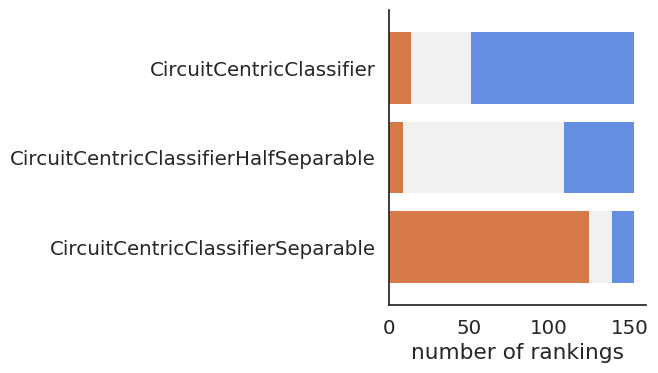
\includegraphics[width=0.82\linewidth]{../plot/figures/ranking-all.png}
    \caption{Number of rankings (blue/first to red/last) across all datasets on which each model was tested, for the three CCC model families. The models are ordered from top to bottom by average normalized rank.}
    \label{fig:ccc-ranking-all}
\end{figure}

Relative to the original CCC, the half-separable variant shows only a small mean loss in test accuracy across the completed benchmark set, about \(-0.0116\). By contrast, the fully separable model is markedly worse, with a mean test-accuracy difference of about \(-0.1705\) relative to the original CCC. This can be seen in Figure~\ref{fig:ccc-forest-diffs}. The difference between the half-separable and fully separable variants is then correspondingly large, about \(+0.1590\) in favor of the half-separable model. The main empirical pattern is therefore not that every reduction of entanglement is equally harmful, but that removing entanglement entirely is much more damaging than thinning it out.

\begin{figure}[H]
    \centering
    \includegraphics[width=0.49\linewidth]{../plot/figures/forest-ccc-half-minus-ccc.png}%
    \includegraphics[width=0.49\linewidth]{../plot/figures/forest-ccc-separable-minus-ccc.png}\par\vspace{-0.8\baselineskip}
    \caption{Forest plots of paired mean test-accuracy differences for the dequantized CCC variants relative to the original CCC. Each point is the average benchmark-wise test-accuracy difference within a family, and each horizontal interval shows the corresponding 95\% confidence interval across matched benchmark instances. Negative values indicate worse performance than the original CCC. The horizontal scales differ between the two panels.}
    \label{fig:ccc-forest-diffs}
\end{figure}

\begin{figure}[htbp]
    \centering
    \parbox[t]{0.47\linewidth}{\centering \small \textbf{Linearly Separable}\par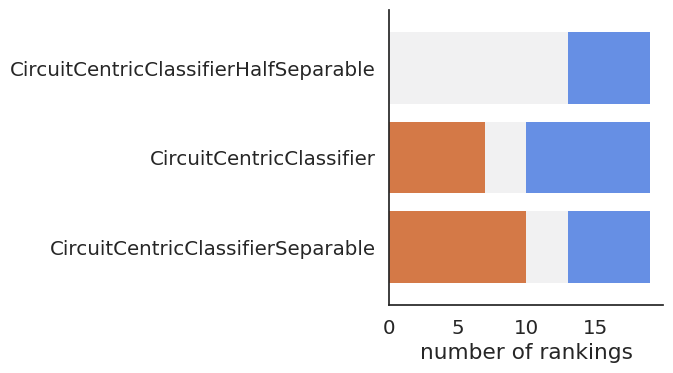
\includegraphics[width=0.96\linewidth]{../plot/figures/ranking-linearly-separable.png}}
    \parbox[t]{0.47\linewidth}{\centering \small \textbf{Hidden Manifold}\par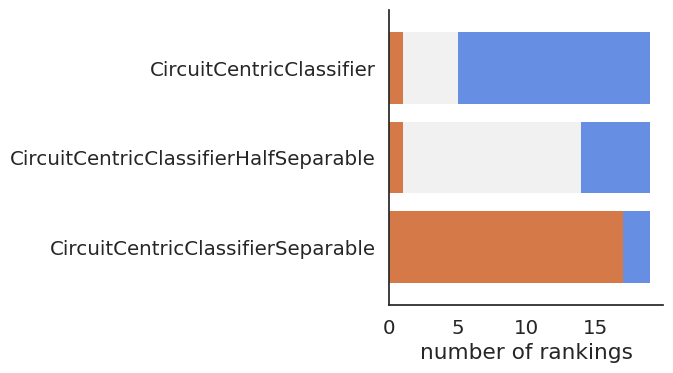
\includegraphics[width=0.96\linewidth]{../plot/figures/ranking-hidden-manifold.png}}
    \parbox[t]{0.47\linewidth}{\centering \small \textbf{Hidden Manifold Diff}\par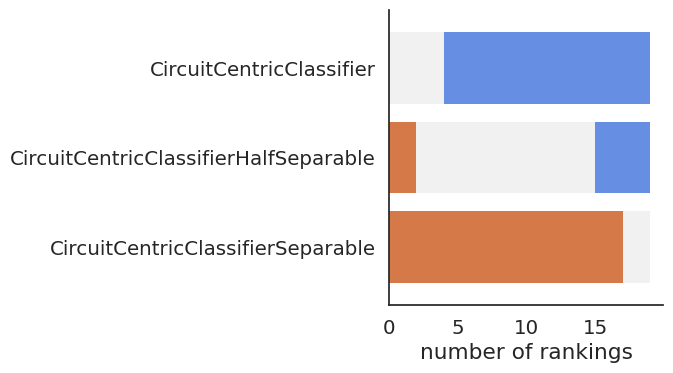
\includegraphics[width=0.96\linewidth]{../plot/figures/ranking-hmm-diff.png}}
    \parbox[t]{0.47\linewidth}{\centering \small \textbf{Hyperplanes Diff}\par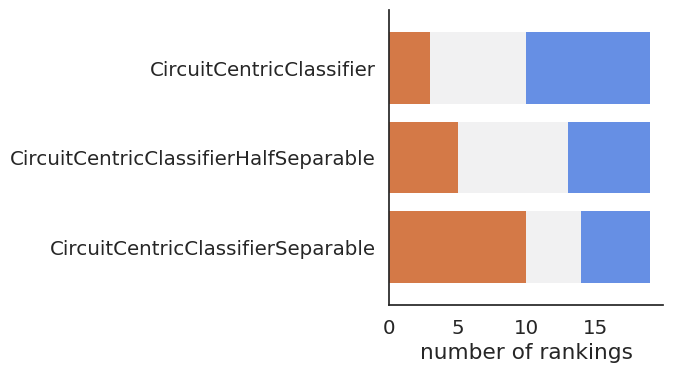
\includegraphics[width=0.96\linewidth]{../plot/figures/ranking-hyperplanes-diff.png}}
    \parbox[t]{0.47\linewidth}{\centering \small \textbf{MNIST PCA}\par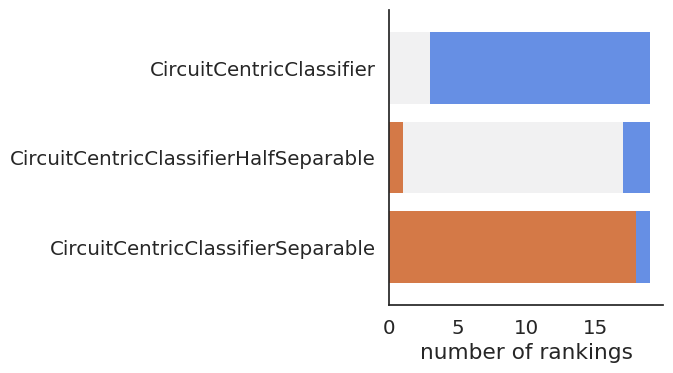
\includegraphics[width=0.96\linewidth]{../plot/figures/ranking-mnist-pca.png}}
    \parbox[t]{0.47\linewidth}{\centering \small \textbf{MNIST PCA Small}\par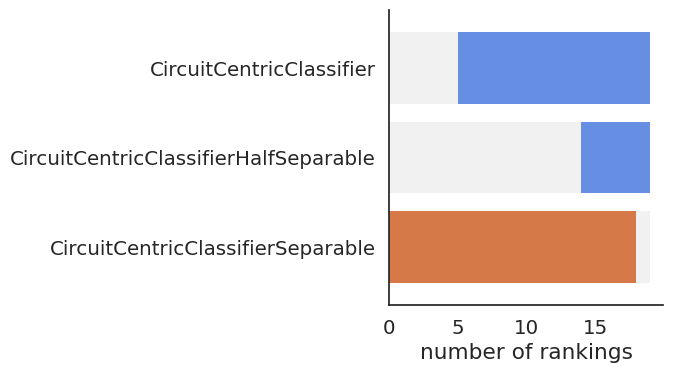
\includegraphics[width=0.96\linewidth]{../plot/figures/ranking-mnist-pca-small.png}}
    \parbox[t]{0.47\linewidth}{\centering \small \textbf{Two Curves}\par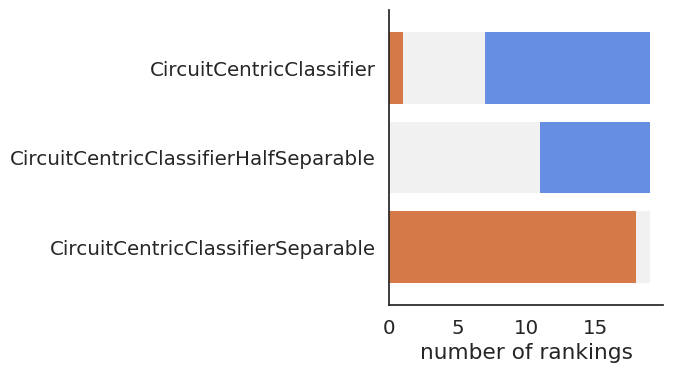
\includegraphics[width=0.96\linewidth]{../plot/figures/ranking-two-curves.png}}
    \parbox[t]{0.47\linewidth}{\centering \small \textbf{Two Curves Diff}\par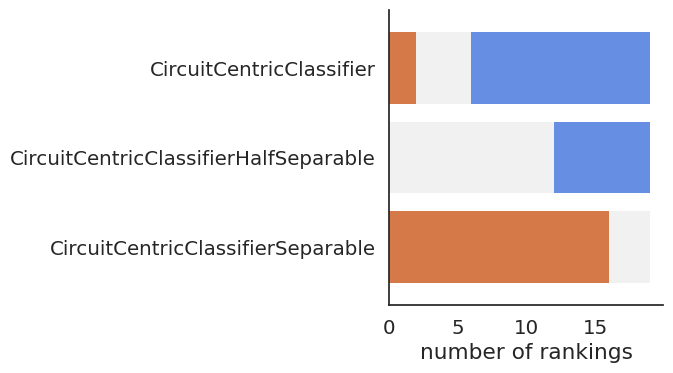
\includegraphics[width=0.96\linewidth]{../plot/figures/ranking-two-curves-diff.png}}
    \caption{Per-family ranking plots for all completed benchmark families: linearly separable, hidden manifold, hidden manifold diff, hyperplanes diff, MNIST PCA, MNIST PCA small, two curves, and two curves diff.}
    \label{fig:ccc-ranking-all-families}
\end{figure}

\begin{figure}[htbp]
    \centering
    \parbox[t]{0.47\linewidth}{\centering \small \textbf{Linearly Separable}\par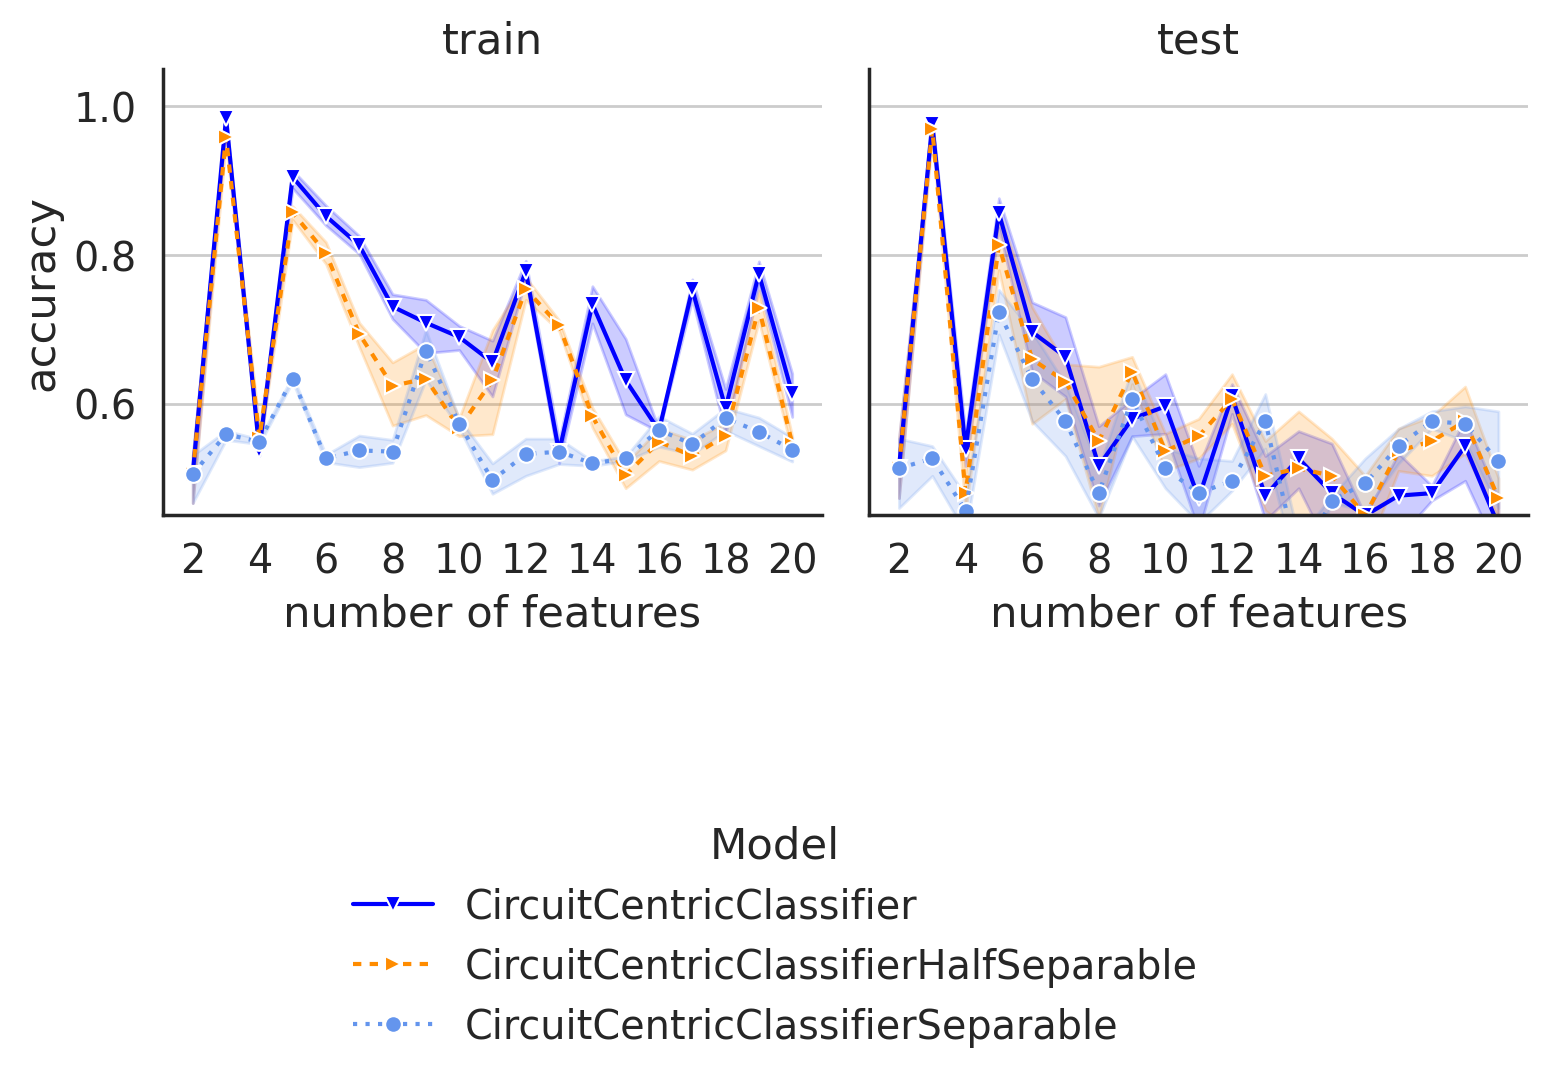
\includegraphics[width=0.96\linewidth]{../plot/figures/score-linearly_separable-ccc-qnn.png}}
    \parbox[t]{0.47\linewidth}{\centering \small \textbf{Hidden Manifold}\par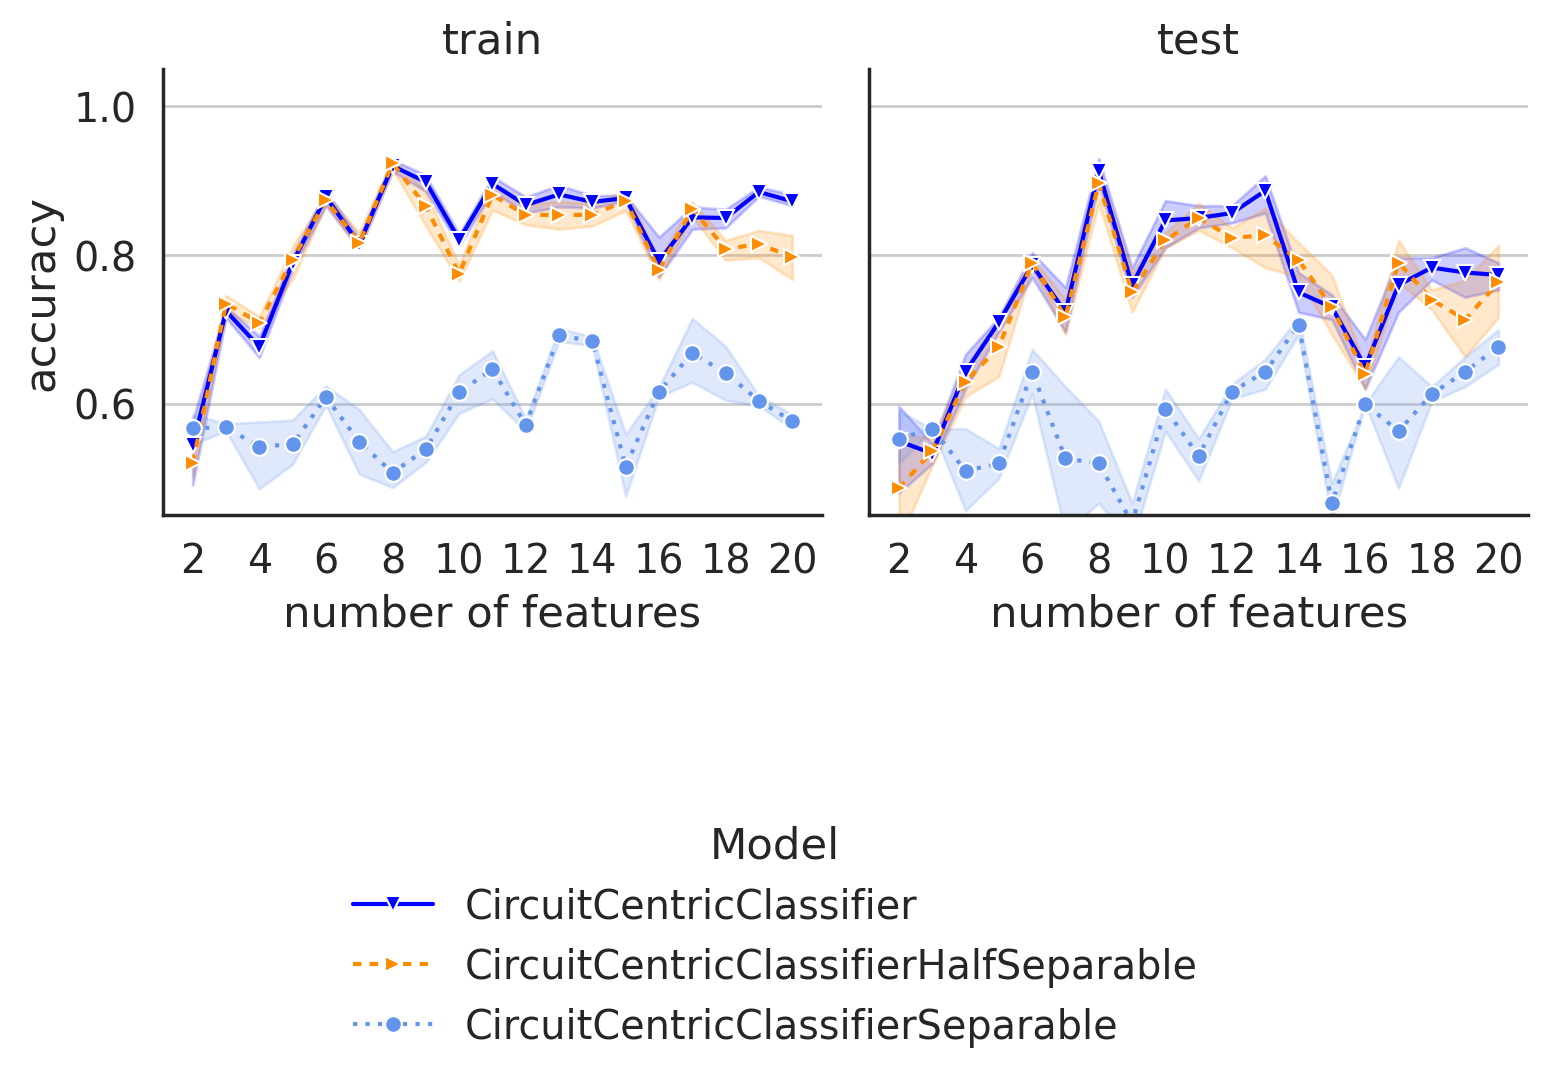
\includegraphics[width=0.96\linewidth]{../plot/figures/score-hidden_manifold-qnn.png}}
    \parbox[t]{0.47\linewidth}{\centering \small \textbf{Hidden Manifold Diff}\par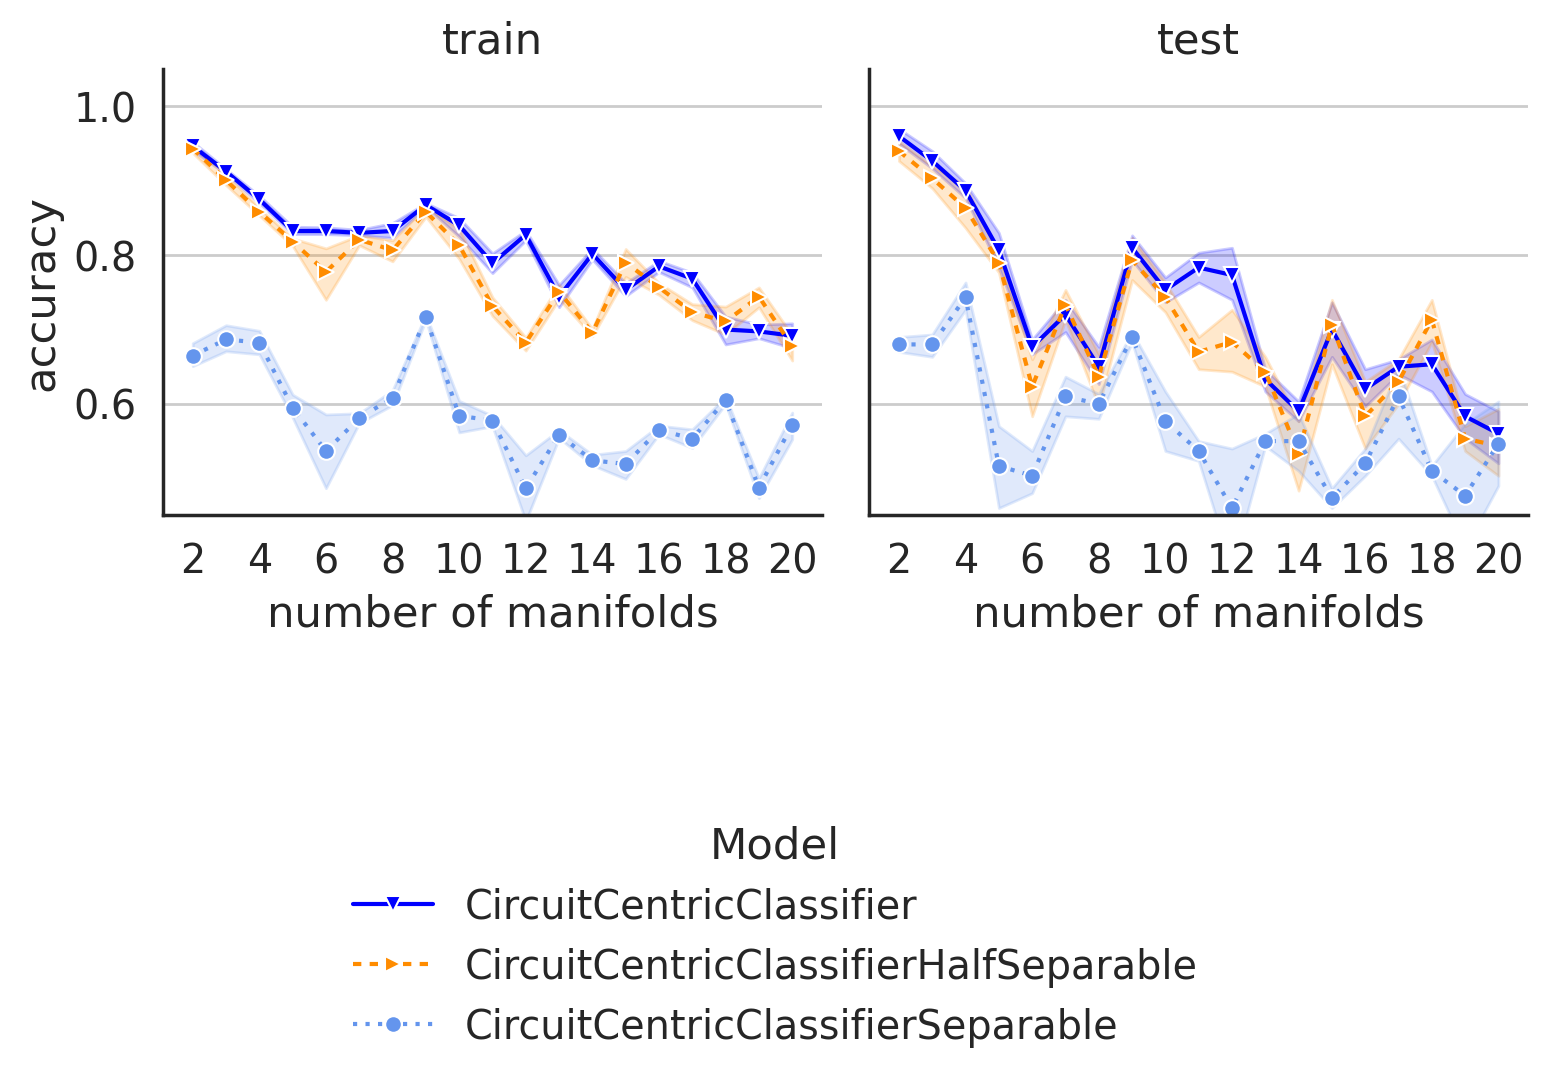
\includegraphics[width=0.96\linewidth]{../plot/figures/score-hidden_manifold_diff-qnn.png}}
    \parbox[t]{0.47\linewidth}{\centering \small \textbf{Hyperplanes Diff}\par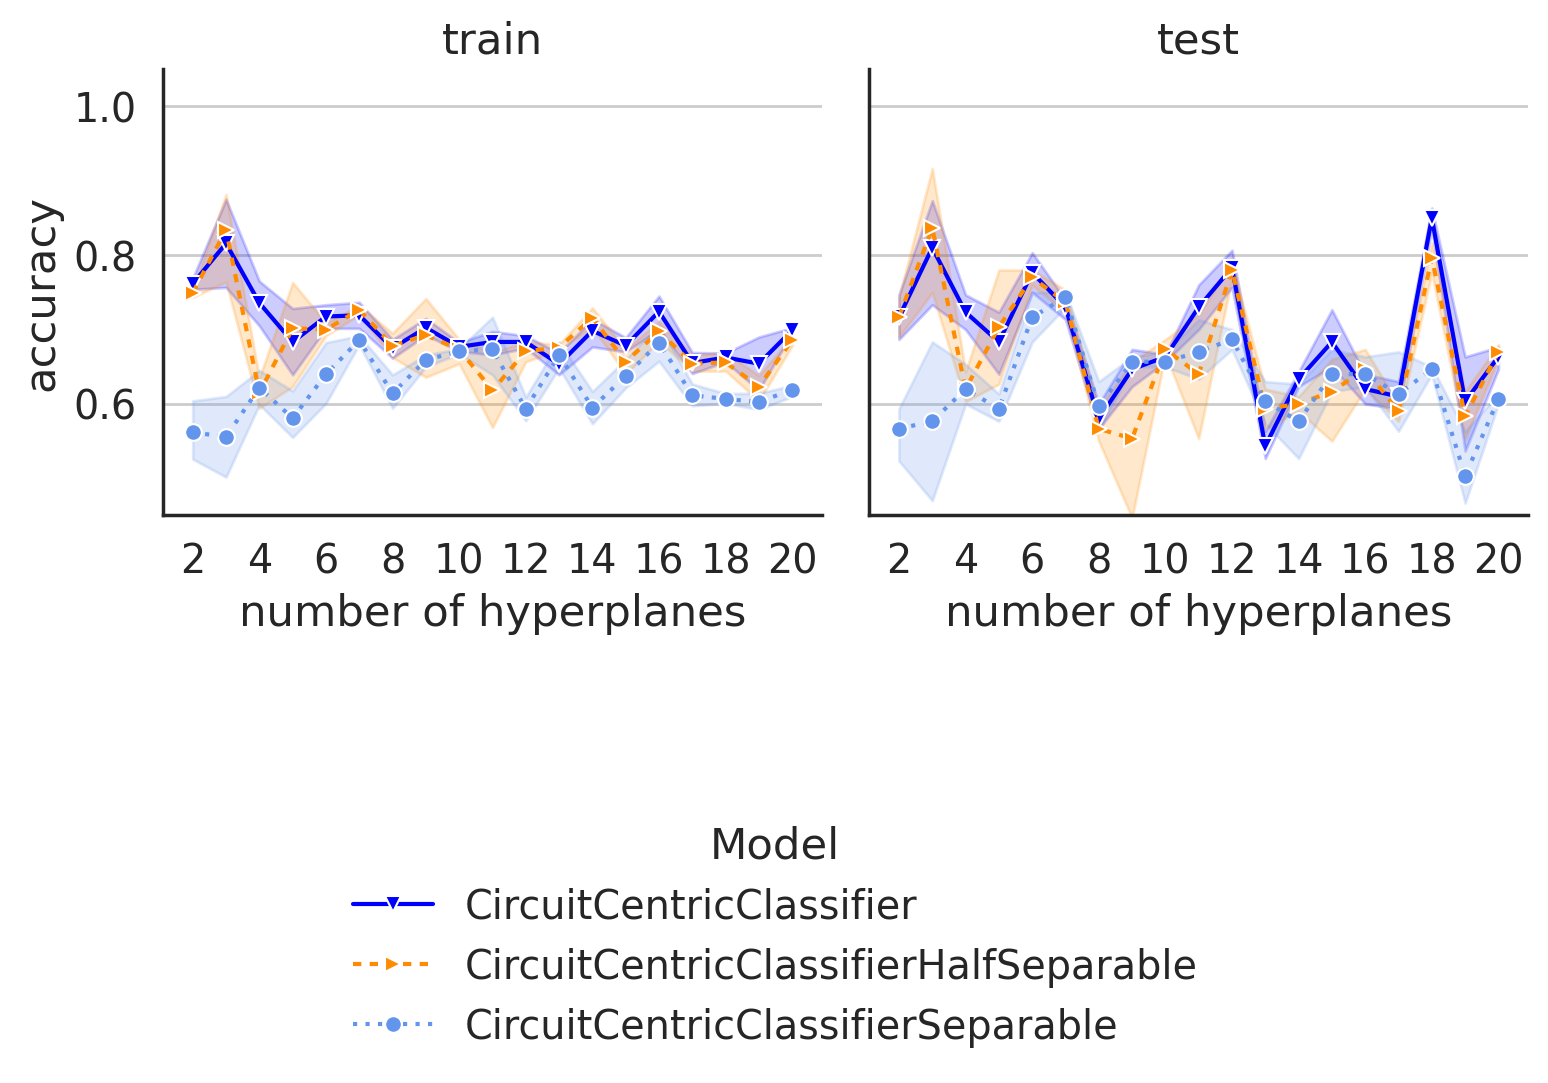
\includegraphics[width=0.96\linewidth]{../plot/figures/score-hyperplanes_diff-qnn.png}}
    \parbox[t]{0.47\linewidth}{\centering \small \textbf{MNIST PCA}\par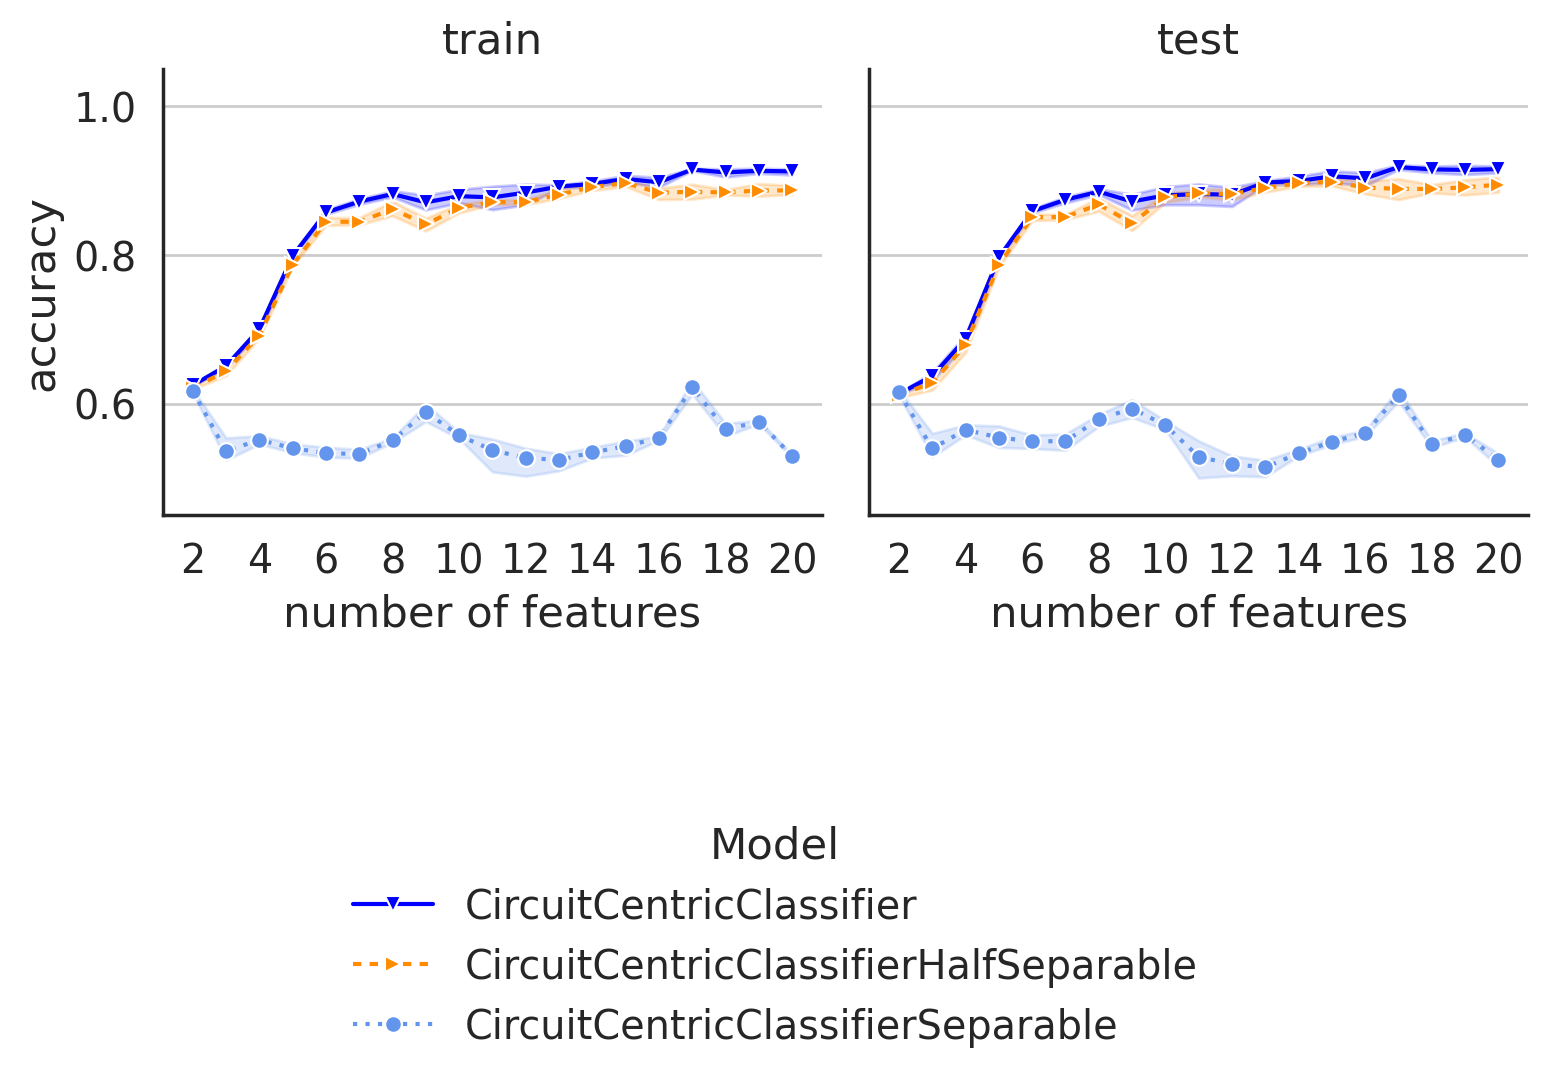
\includegraphics[width=0.96\linewidth]{../plot/figures/score-mnist_pca-qnn.png}}
    \parbox[t]{0.47\linewidth}{\centering \small \textbf{MNIST PCA Small}\par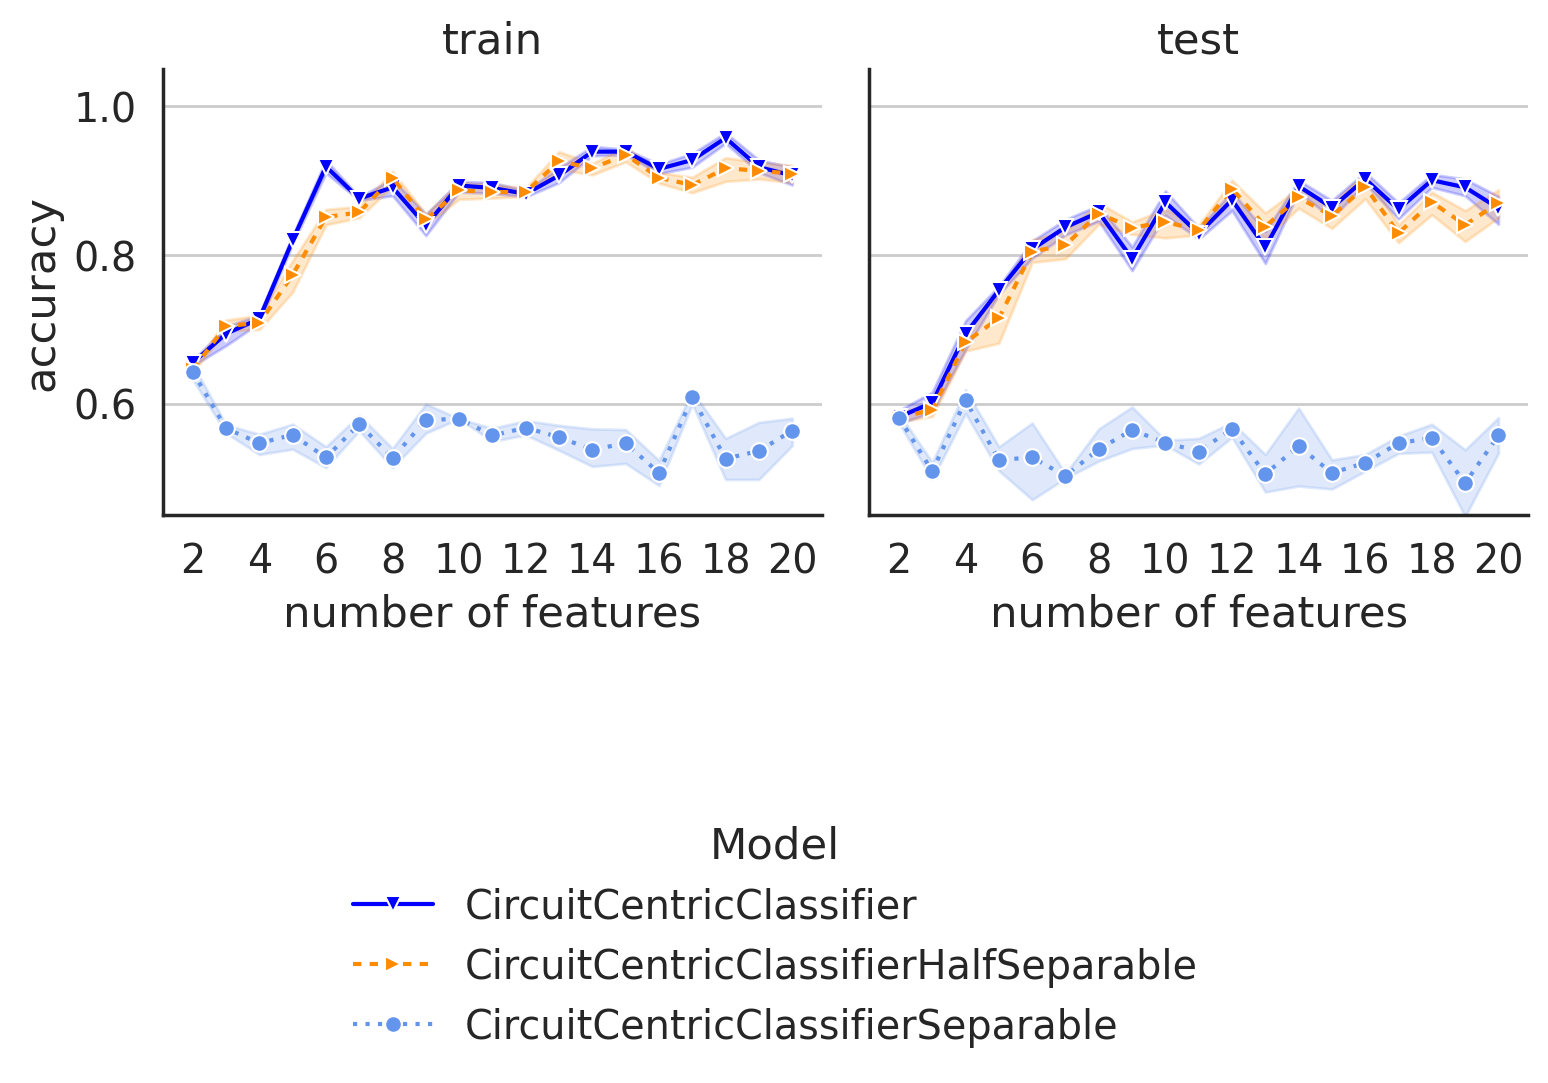
\includegraphics[width=0.96\linewidth]{../plot/figures/score-mnist_pca--qnn.png}}
    \parbox[t]{0.47\linewidth}{\centering \small \textbf{Two Curves}\par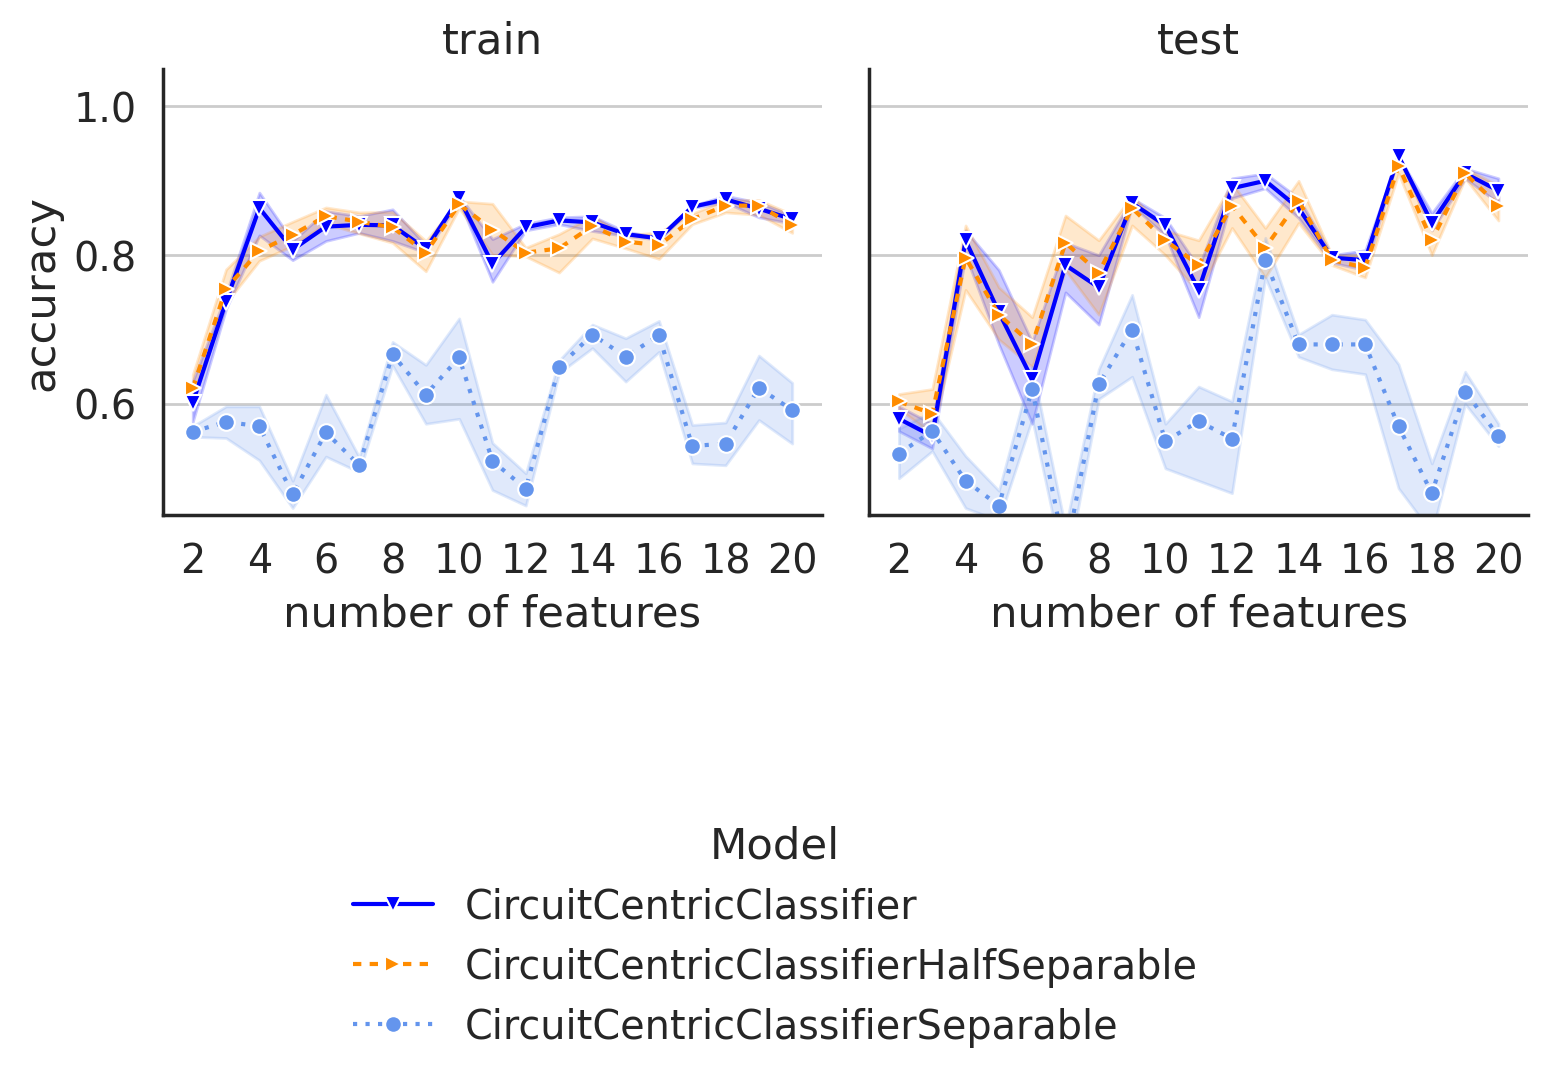
\includegraphics[width=0.96\linewidth]{../plot/figures/score-two_curves-qnn.png}}
    \parbox[t]{0.47\linewidth}{\centering \small \textbf{Two Curves Diff}\par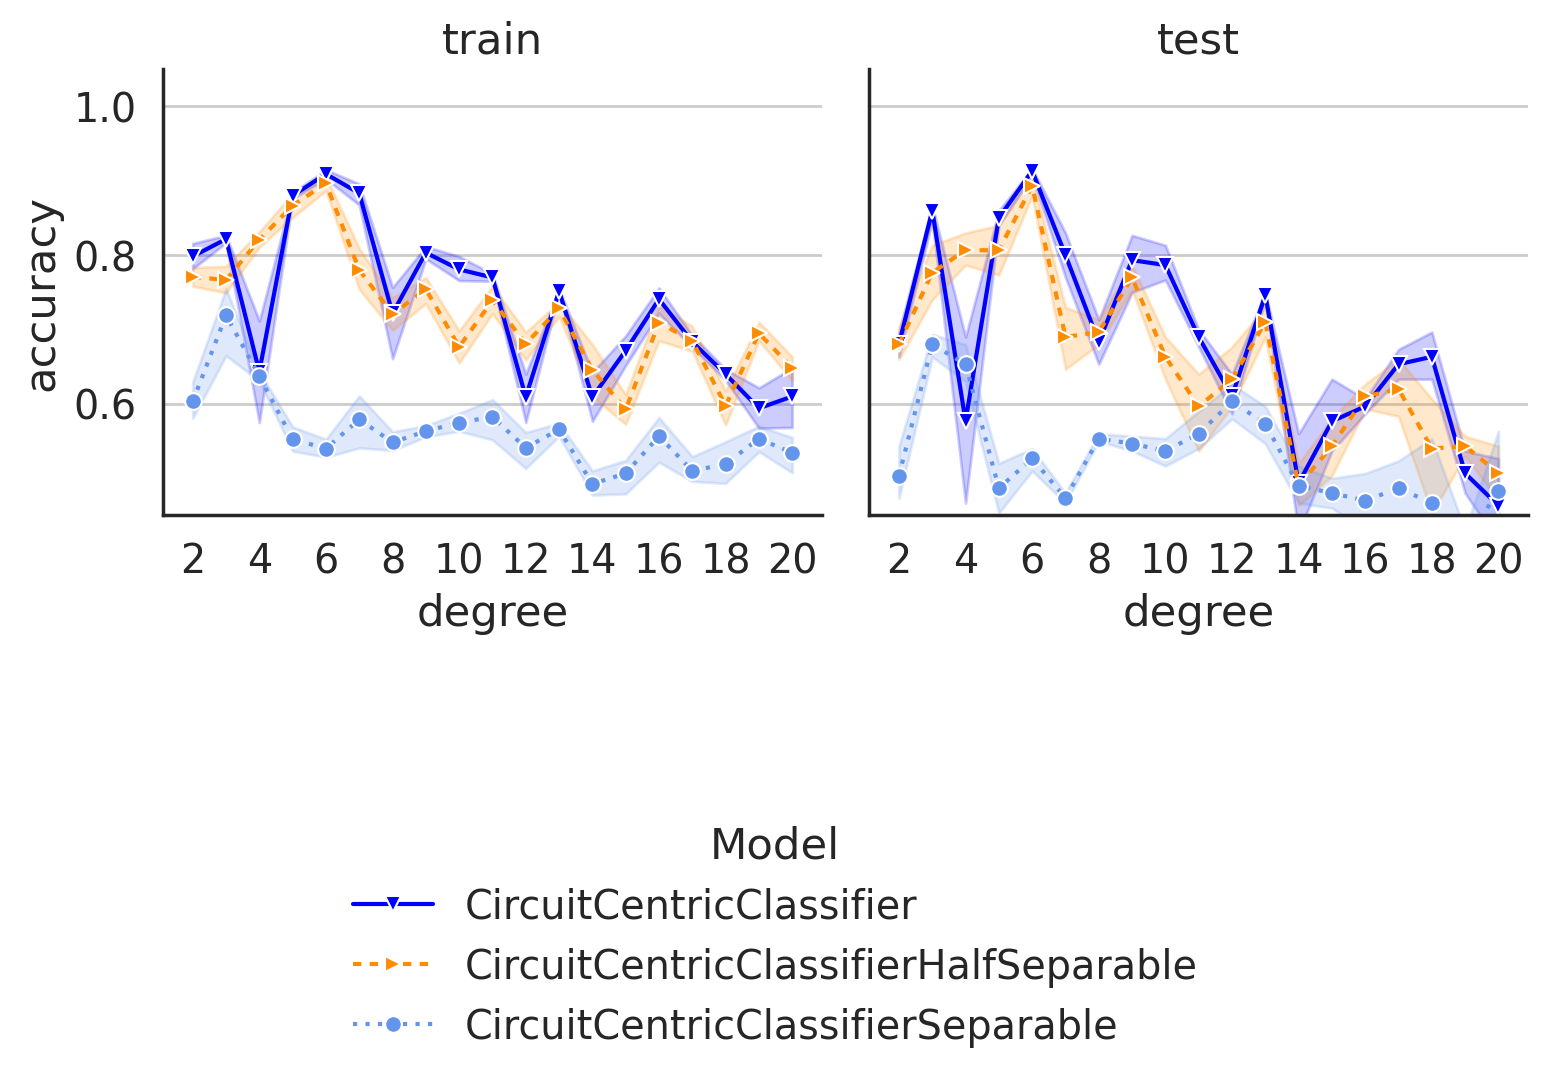
\includegraphics[width=0.96\linewidth]{../plot/figures/score-two_curves_diff-qnn.png}}
    \caption{Train and test accuracy curves for all completed benchmark families: linearly separable, hidden manifold, hidden manifold diff, hyperplanes diff, MNIST PCA, MNIST PCA small, two curves, and two curves diff.}
    \label{fig:ccc-scores-all}
\end{figure}


This pattern is also visible when the results are broken down by benchmark family, as shown by the forest plots in Figure~\ref{fig:ccc-forest-diffs}. On linearly separable data, the half-separable variant is slightly better on average than the original model, by about \(+0.0091\), while the fully separable model is slightly worse, by about \(-0.0391\). This suggests that for the simplest tasks in the completed benchmark set, the full entangling structure may not be necessary. On hyperplanes diff, the three variants are comparatively close, with the separable model behind the original by only about \(-0.0598\). By contrast, on hidden manifold, hidden manifold diff, MNIST PCA, MNIST PCA small, and two curves diff, the fully separable model is consistently and often substantially worse than the original CCC. The effect is especially pronounced on the MNIST PCA families, where the separable model trails the original by about \(-0.2934\) and \(-0.2765\), respectively.

The half-separable variant occupies an intermediate position. On most benchmark families it is slightly worse than the original CCC, but the drop is small compared with the fully separable case. For example, the average test-accuracy difference half-minus-full is about \(-0.0163\) on hidden manifold, \(-0.0237\) on hidden manifold diff, \(-0.0188\) on hyperplanes diff, \(-0.0124\) on MNIST PCA, \(-0.0088\) on MNIST PCA small, and \(-0.0193\) on two curves diff. These values are modest enough to suggest that, across the completed CCC benchmark families, a sparse entangling structure retains a substantial fraction of the original model's performance, which is also reflected in the train and test curves shown in Figure~\ref{fig:ccc-scores-all}.

The train-versus-test comparison is broadly consistent with this interpretation. Averaged over the completed benchmark set, the original CCC reaches about 0.7886 train accuracy and 0.7347 test accuracy, while the half-separable variant reaches about 0.7698 train accuracy and 0.7232 test accuracy. The separable model is much lower on both metrics, with about 0.5775 train accuracy and 0.5642 test accuracy. In other words, the separable model does not merely generalize worse after fitting the data equally well; it appears to have substantially lower effective fitting capacity on these tasks. This can be seen in Table~\ref{tab:ccc-train-test-gaps}.

\begin{table}[htbp]
\centering
\small
\setlength{\tabcolsep}{4pt}
\resizebox{\textwidth}{!}{%
\begin{tabular}{l|ccc|ccc|ccc}
\hline
\rowcolor{gray!20}
Benchmark &
\multicolumn{3}{c|}{\textbf{CCC}} &
\multicolumn{3}{c|}{\textbf{Half-Sep}} &
\multicolumn{3}{c}{\textbf{Sep}} \\
\rowcolor{gray!12}
&
Train & Test & Gap &
Train & Test & Gap &
Train & Test & Gap \\
\hline
\rowcolor{gray!4}
Linearly Separable   & \cellcolor{blue!45}0.703 & \cellcolor{blue!20}0.573 & \cellcolor{orange!45}0.130 & \cellcolor{blue!30}0.647 & \cellcolor{blue!20}0.582 & \cellcolor{orange!22}0.064 & \cellcolor{blue!18}0.553 & \cellcolor{blue!15}0.534 & \cellcolor{orange!8}0.018 \\
Hidden Manifold      & \cellcolor{blue!78}0.827 & \cellcolor{blue!58}0.752 & \cellcolor{orange!26}0.075 & \cellcolor{blue!72}0.810 & \cellcolor{blue!54}0.735 & \cellcolor{orange!26}0.075 & \cellcolor{blue!22}0.593 & \cellcolor{blue!18}0.575 & \cellcolor{orange!8}0.017 \\
\rowcolor{gray!4}
Hidden Manifold Diff & \cellcolor{blue!72}0.807 & \cellcolor{blue!50}0.723 & \cellcolor{orange!30}0.084 & \cellcolor{blue!65}0.782 & \cellcolor{blue!43}0.699 & \cellcolor{orange!29}0.083 & \cellcolor{blue!21}0.584 & \cellcolor{blue!17}0.570 & \cellcolor{orange!7}0.014 \\
Hyperplanes Diff     & \cellcolor{blue!44}0.699 & \cellcolor{blue!39}0.687 & \cellcolor{orange!5}0.012 & \cellcolor{blue!39}0.686 & \cellcolor{blue!34}0.668 & \cellcolor{orange!8}0.017 & \cellcolor{blue!26}0.625 & \cellcolor{blue!26}0.627 & \cellcolor{orange!3}-0.002 \\
\rowcolor{gray!4}
MNIST PCA            & \cellcolor{blue!85}0.849 & \cellcolor{blue!85}0.850 & \cellcolor{orange!3}-0.000 & \cellcolor{blue!80}0.834 & \cellcolor{blue!81}0.837 & \cellcolor{orange!3}-0.003 & \cellcolor{blue!18}0.554 & \cellcolor{blue!18}0.556 & \cellcolor{orange!3}-0.002 \\
MNIST PCA Small      & \cellcolor{blue!88}0.868 & \cellcolor{blue!73}0.815 & \cellcolor{orange!18}0.053 & \cellcolor{blue!83}0.856 & \cellcolor{blue!70}0.807 & \cellcolor{orange!17}0.050 & \cellcolor{blue!19}0.559 & \cellcolor{blue!16}0.539 & \cellcolor{orange!8}0.020 \\
\rowcolor{gray!4}
Two Curves           & \cellcolor{blue!76}0.823 & \cellcolor{blue!69}0.797 & \cellcolor{orange!10}0.026 & \cellcolor{blue!75}0.819 & \cellcolor{blue!68}0.794 & \cellcolor{orange!10}0.024 & \cellcolor{blue!21}0.590 & \cellcolor{blue!19}0.586 & \cellcolor{orange!4}0.004 \\
Two Curves Diff      & \cellcolor{blue!52}0.733 & \cellcolor{blue!37}0.681 & \cellcolor{orange!17}0.051 & \cellcolor{blue!49}0.725 & \cellcolor{blue!32}0.662 & \cellcolor{orange!22}0.063 & \cellcolor{blue!18}0.562 & \cellcolor{blue!14}0.526 & \cellcolor{orange!12}0.036 \\
\hline
\end{tabular}
}
\caption{Family-level averages of train accuracy, test accuracy, and train-test gap for the three CCC variants across the completed benchmark set. Darker blue indicates higher accuracy; darker orange indicates a larger train-test gap. The gap is defined as train minus test.}
\label{tab:ccc-train-test-gaps}
\end{table}


The main quantitative conclusion from the completed CCC data is the following: the original entangling CCC is usually best, but the half-separable variant remains competitive, whereas the fully separable model often incurs a substantial loss. Entanglement appears to matter in this benchmark setting, but the completed results suggest that full entangler density is often not required to obtain most of the performance of the original model on the tasks studied here.

\section{Qualitative Interpretation}

The dataset families probe different kinds of structure, and the effect of entanglement is not uniform across them.

The linearly separable benchmark primarily tests whether a model can recover a simple hyperplane-based decision rule; a task a simple linear classifier should be able to do. Since this structure does not require complex nonlinear or compositional feature interactions, small differences between the CCC variants on this family are consistent with the expectation that strong entangling connectivity is not central for this task. However, the relatively modest absolute accuracies limit the strength of this interpretation. In particular, the slight advantage of the half-separable variant over the original CCC should not be over-interpreted as evidence against the usefulness of entanglement more broadly. The task may be simple enough that the full entangling structure provides more representational capacity than necessary, potentially leading to overfitting. This interpretation is supported by the larger train--test gap observed for the original CCC, which is the largest among all.

The hidden-manifold families tell a different story. There the fully separable model drops substantially, while the original and half-separable variants remain much closer. Since these benchmarks are intended to probe structure that is embedded nontrivially in a larger feature space; both as the hidden structure complexity remains constant and the feature dimensions grow in number and vice versa, the found pattern is consistent with the idea that some nonlocal interaction structure in the variational block helps the model align with the task. 

Similarly, MNIST PCA families show a particularly pronounced degradation of the fully separable model relative to the original CCC and the half-separable variant. Although the separable model also performs poorly on linearly separable and two-curves-diff benchmarks, those families are challenging for the entangling variants as well. The MNIST PCA case is therefore more distinctive, because the performance loss appears especially specific to the fully separable architecture. One possible explanation is that MNIST PCA retains distributed image-like structure, where class-relevant information is spread across several input components. Without entangling operations, this information cannot be effectively mixed across qubits before the final first-qubit measurement, making the separable variant particularly susceptible to an architectural bottleneck.

The standard two-curves benchmark shows a qualitatively similar pattern to the MNIST PCA families: removing entanglement entirely leads to a pronounced degradation of the fully separable model, while the half-separable variant remains much closer to the original CCC. The two-curves-diff benchmark, however, should be interpreted separately. Its lower performance for the original CCC and the half-separable variant can be attributed to the construction of the task itself. While the standard two-curves benchmark keeps the curve complexity fixed, two-curves-diff increases the geometric complexity of the underlying curves at fixed feature dimension. The resulting decision structure is more intricate and may require the model to capture more oscillatory nonlinear relations between features. Therefore, the reduced performance of the entangling variants on two-curves-diff is better understood as reflecting the intrinsic difficulty of the benchmark, rather than only the effect of entanglement reduction.

The results for the hyperplanes diff benchmark show a somewhat different pattern from the other benchmark families. For the CCC and HalfSeparable models, which both retain entangling operations to different degrees, hyperplanes diff performs relatively poorly compared with the other benchmarks. In contrast, the fully separable model performs comparatively well on this benchmark. One possible explanation is that this task depends less on learning rich entangled feature interactions and more on combining several local boundary relations. In this setting, the local rotations of the separable model may still be sufficient to capture a substantial part of the repeated hyperplane structure. To provide a contrast example, in hidden manifold diff, the hidden structure governing the data becomes richer and more complex, and in two curves diff, the Fourier degree increases, making the curves more oscillatory and geometrically intricate. Therefore, the classifier may need to integrate information across multiple dimensions or regions simultaneously. These properties would be expected to suffer more strongly when entanglement is removed.

Furthermore, although a small train-test gap can indicate good generalization, low train and test accuracies together more commonly suggest underfitting. This behavior appears repeatedly for the fully separable variant. This could be caused by the architectural limitation of the separable variant for which the measurement procedure remains on only the first qubit. Without entangling operations, information from distant qubits may therefore influence the output less effectively, introducing an architectural bottleneck. Overall, the train-test evidence suggests that removing entanglement entirely weakens the model primarily by reducing its ability to fit the tasks, whereas partial entanglement preserves much of that fitting capacity.

The benchmark-family averages do not show a uniform relationship between overall performance and the difference in the train--test gap between the CCC and half-separable variants. There is some tendency for stronger-performing families to exhibit smaller gap differences between the two models, but this pattern is not consistent across all benchmark families. In particular, the linearly separable benchmark stands out, while several other families show only very small gap differences regardless of their absolute performance level. The observed correlation therefore depends strongly on the small number of benchmark families considered, and especially on the linearly separable case. When this benchmark is excluded, the correlation becomes much weaker. Thus, the evidence suggests, at most, a mild trend rather than a robust general relationship, or simply that benchmarks with better average test accuracies have in general low degradation and therefore low difference between gaps.

\section{Limitations} 
The results of this thesis should be interpreted within several important limitations. 

First, all experiments were performed in a simulation-based setting. The reported results therefore characterize the behavior of the implemented model architectures under idealized simulator conditions, but they do not account for hardware-specific effects such as gate noise, finite-shot sampling, decoherence, calibration errors, or restricted device connectivity. Consequently, the experiments should not be interpreted as direct evidence of performance on present-day quantum hardware. 

A second limitation concerns the type of data considered. The benchmark families used in this thesis consist of classical datasets that are embedded into quantum circuits through encoding procedures such as amplitude encoding or feature maps. This differs from quantum-dataset settings, where the data may consist directly of quantum states generated by quantum processes \parencite{schatzki2021entangled} or, more broadly, data generated by or characterizing quantum systems, such as state vectors, Hamiltonians, unitaries, measurement distributions, control pulses, and noise information \parencite{perrier2021qdataset}. The present work therefore studies quantum models applied to classical learning problems, rather than learning directly from intrinsically quantum-mechanical data obtained from physical or simulated quantum systems.

The scope of the model comparison is also limited. The main empirical analysis focuses on the Circuit-Centric Classifier and its entanglement-reduced variants, with only limited results available for the IQP kernel family. The conclusions should therefore not be understood as statements about quantum machine learning models in general. They apply specifically to the evaluated model families, benchmark tasks, and implementation choices. Similarly, the entanglement reduction studied here follows one particular controlled ablation strategy based on removing or sparsifying two-qubit couplings. Other dequantization strategies, different ansatz designs, or alternative measurement rules could lead to different behavior. 

A further architectural limitation is specific to the CCC model. The prediction rule measures only the Pauli-\(Z\) expectation value of the first qubit. In the original and partially entangling variants, entangling gates allow information from other qubits to influence this measured output qubit. In the fully separable variant, this information transfer is removed. As a result, part of the poor performance of the separable CCC may reflect a measurement bottleneck rather than only the absence of entanglement itself. Modifying the measurement rule could mitigate this issue, but it would constitute a more invasive architectural change than the entanglement ablation considered in this thesis. 

The benchmark coverage is also constrained by computational resources, which were directly tied to the finite compute-time allocation available for the RWTH Aachen HPC project used in this thesis. Since the project quota limited the total number of CPU core-hours available for dataset generation, hyperparameter searches, and repeated scoring runs, not all planned experiments could be completed at the same scale. This particularly affected some benchmark families from the reference suite, such as bars-and-stripes, and the IQP kernel experiments. As for which quantum kernel evaluation requires constructing pairwise kernel matrices and therefore scales unfavorably with dataset size and hyperparameter settings. 

Finally, the results remain subject to the usual limitations of empirical benchmarking. Performance can depend on the selected hyperparameter search space, optimization settings, random seeds, and evaluation metric. For this matter, selection followed \parencite{bowles2024better}.  Although repeated runs and fixed seeds were used to improve reproducibility, the analysis is still based on a finite number of experiments. Therefore, statistical variance is expected even with averaging.

\chapter{Conclusion and Outlook}

\nocite{havlicek2019supervised}
\bibliographystyle{apalike}
\bibliography{references}


\end{document}
